%%%%%%%%%%%%%%%%%%%% Preamble %%%%%%%%%%%%%%%%%%%%
\documentclass[10pt, paper=a4]{article}
\usepackage{amssymb,amsfonts,amsmath,latexsym,amsthm, mathtools} %mathtext,
\usepackage{booktabs}
\usepackage{multirow}
\usepackage{graphicx}
\usepackage{listings}
\usepackage{chngpage}
\usepackage{cprotect}
\usepackage[font=footnotesize, labelsep=period]{caption}
\usepackage{cite}
\usepackage[scale=0.925]{geometry}
\graphicspath{{images/}}
\usepackage[pdftex,unicode,colorlinks, citecolor=blue,
  filecolor=black, linkcolor=blue, urlcolor=blue]{hyperref}
\usepackage[figure,table]{hypcap}
%%%%%%%%%%%%%%%%%%%% Document %%%%%%%%%%%%%%%%%%%%
\begin{document}
%%%%%%%%%%%%%%%%%%%% Title page %%%%%%%%%%%%%%%%%%%%
\title{Report 02 --- Regression and classification of age of abalones}

\author{Dmitriy Markovich and Julian Lemos Vinasco}

\date{}

\maketitle

\begin{abstract}
  We solve the regression problem of predicting the age of abalones on
  the basis of its measured physical characteristics, as well as the
  similar classification problem of predicting the age of range of
  abalones.  We consider linear regression, linear regression with
  forward selection, decision trees (DT), k nearest neighbors (KNN),
  naive bayes (NB), artificial neural networks (ANN), and multinomial
  regression (MNMR) methods.  For classification problem, we found the
  ANN and MNMR to be the best performing models, and showed them to
  perform better than the largest class (Lcl) classifier using the
  paired t-test.
  %% Objective: The objective of this second report is to apply the
  %% methods you have learned in the second section of the course on
  %% ”Supervised learning: Classification and regression” in order to
  %% solve both a relevant classification and regression problem for your
  %% data.
\end{abstract}

%%%%%%%%%%%%%%%%%%%% Introduction %%%%%%%%%%%%%%%%%%%%
\section{Regression}
\label{sec:regression}

\subsection{Problem description}
The linear regression objective is to predict the Abalon's age based
on 9 given attributes. The attributes considered for Linear Regression
(LR) are presented next: Sex, Length, Diameter, Height, Whole weight
(WhlWght), Shucked weight (ShckdWght), Viscera weight (VscrWght) and
Shell weight (ShllWght). More details about the data set can be seen
in \cite{datadescription}.

\subsection{Linear Regression with forward selection}
Prior to the LR, the relation between the dependent variable Age and
the independent attibutes was explored by a generalized additive
model. Fig.~\ref{fig:gam} shows that the attributes Length, WhlWght
and ShckdWght do not have a liner relation with Age. The grahps
suggest that exponential terms of this attributes are needed.

\begin{figure}[h]
  \centering
  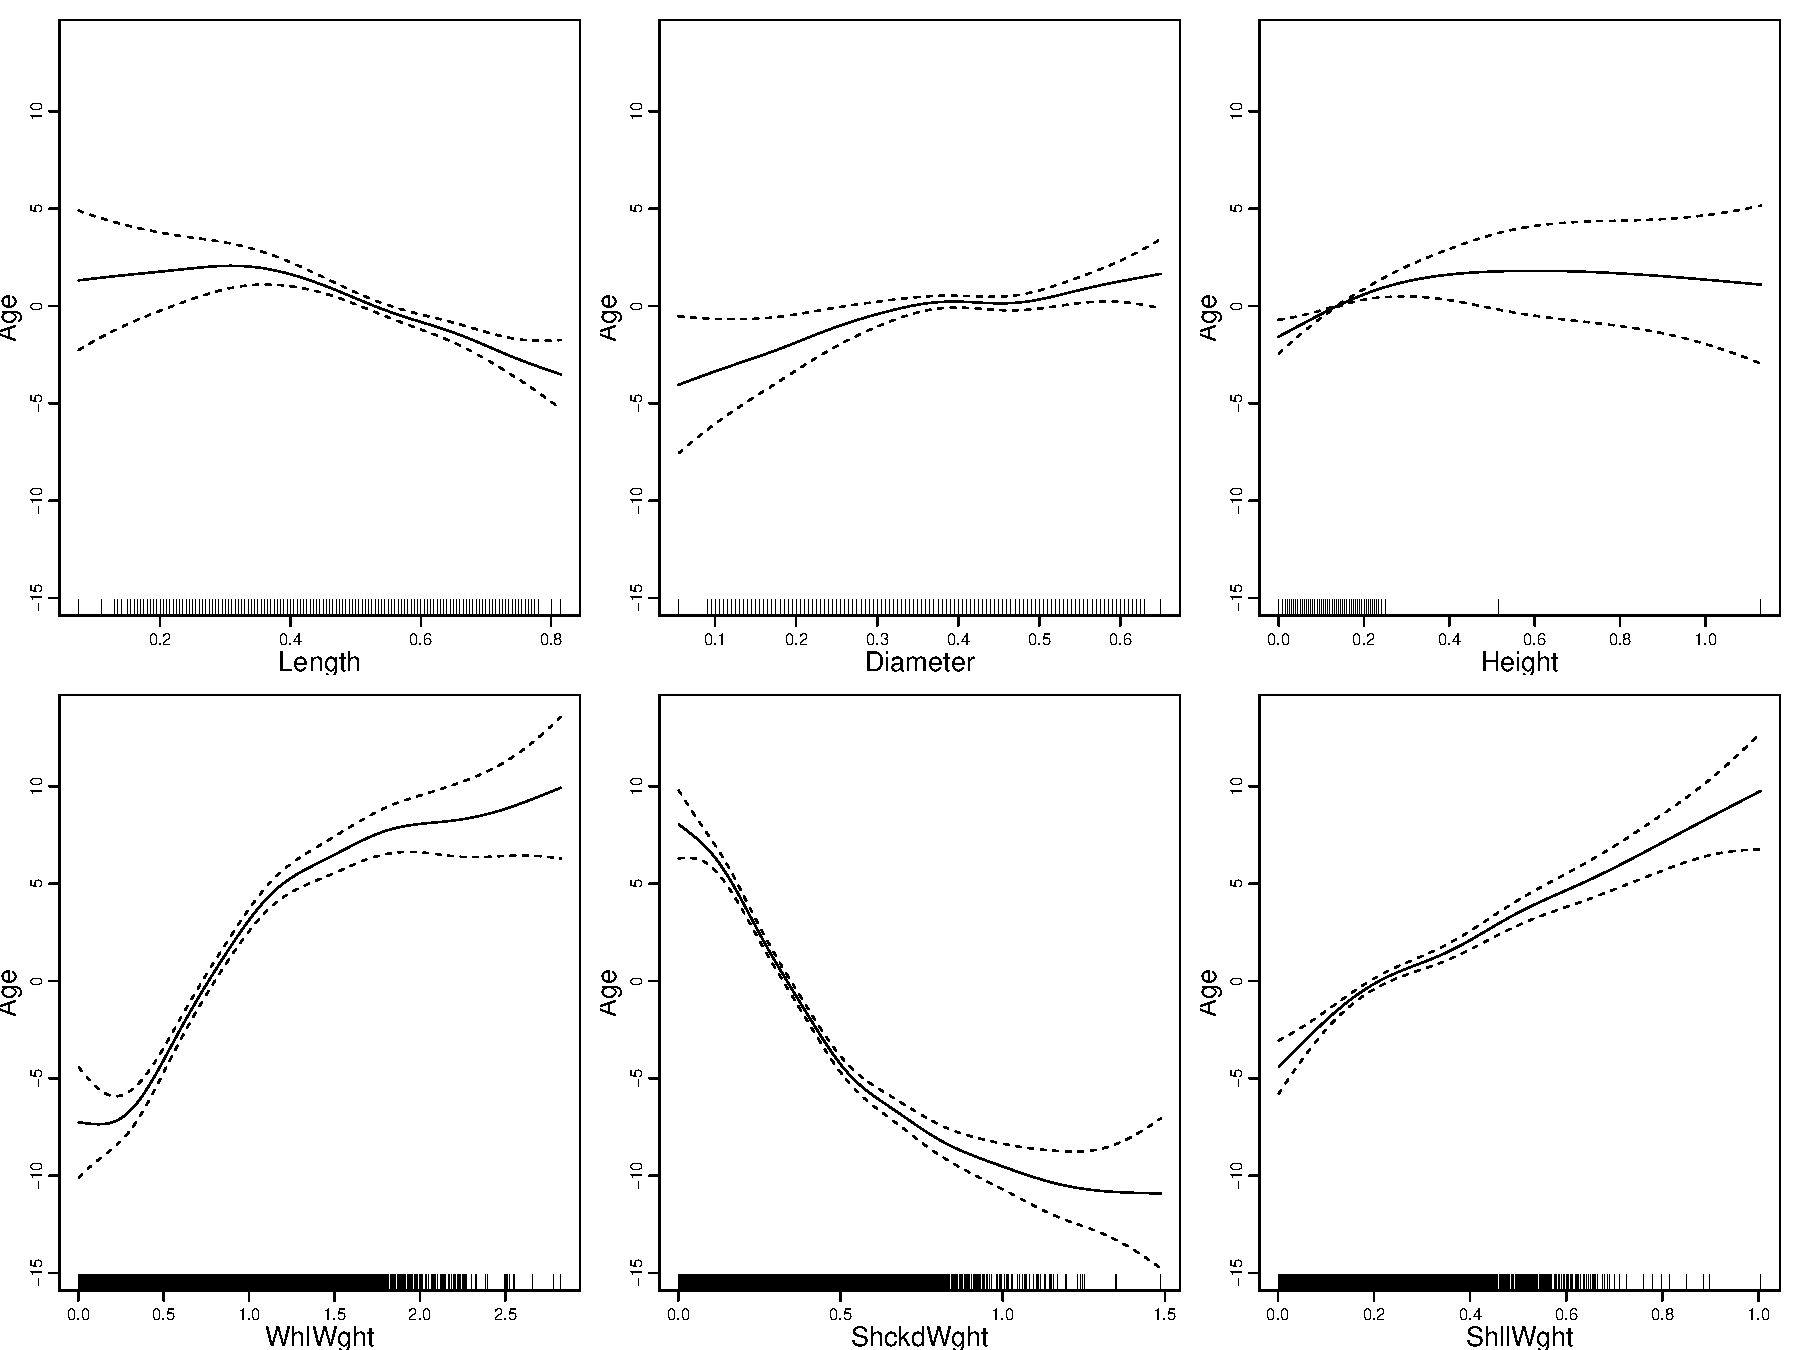
\includegraphics[width = 0.60\textwidth]{gam.pdf}
  \caption{Attributes relation with Age.}
  \label{fig:gam}
\end{figure}

Additionally, an initial LR model was implemented in order to check
the model's assumptions. Fig.~\ref{fig:modelcheck} shows a clearly
trompet shape suggesting the need for a logaritmic transformation of
the response variable Age. Additionally, from the cook's distance it
is clearly that observation 2052 corresponds to and outlier and it
will be removed from the data.

\newpage
\begin{figure}[h]
  \centering
  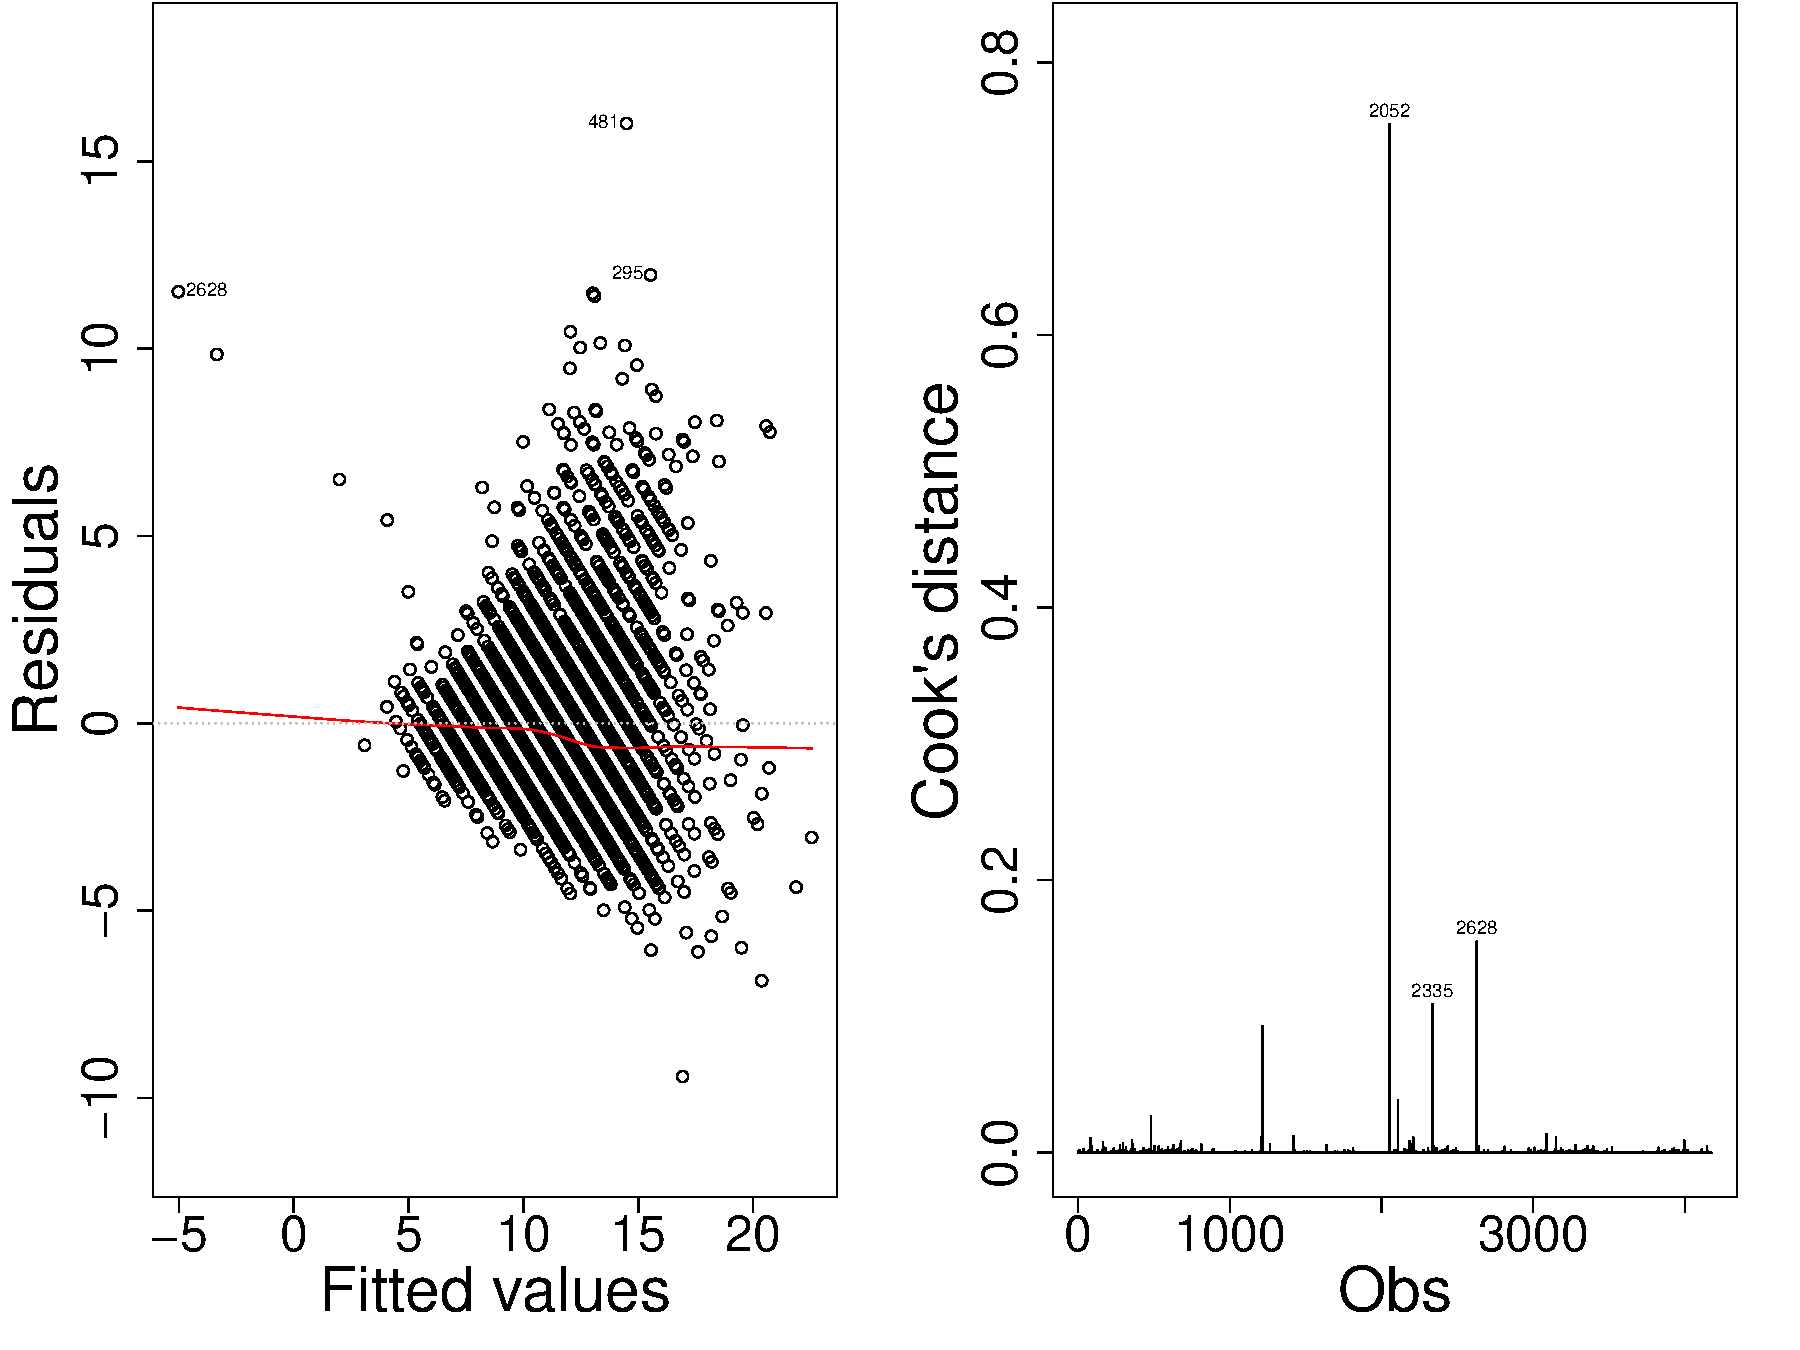
\includegraphics[width = 0.49\textwidth]{modelcheck.pdf}
  \caption{Initial LR normality.}
  \label{fig:modelcheck}
\end{figure}

The forward slection with 10-fold cross-validation to perform
sequential feature selection was implemented considering previous
analysis. Fig.~\ref{fig:forwardselection} shows Squared error and the
attributes selected in each iteration. From the plots it is clear that
the model used in iteration 10 is the one with less error.

\begin{figure}[h]
  \centering
  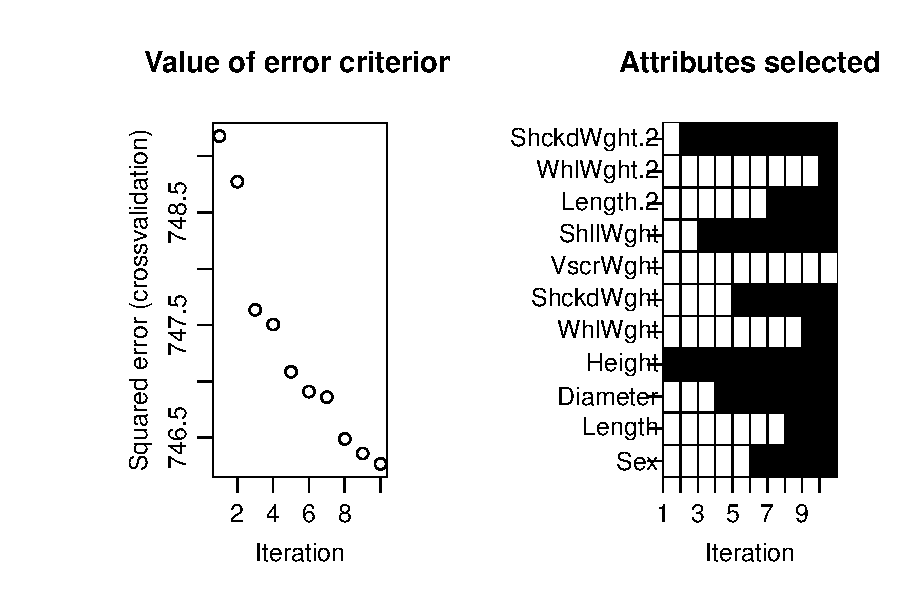
\includegraphics[width = 0.49\textwidth]{forwardselection.pdf}
  \caption{Forward selection results.}
  \label{fig:forwardselection}
\end{figure}

\subsection{Model Interpretation}
The model formulation found in the previous section is presented next:\\

$log(Age)= (Sex + Length + Length^2 + Diameter +Height + WhlWght + WhlWght^2 + ShckdWght + ShckdWght^2 +ShllWght)$\\

Furthermore, the model's coefficients can be seen in
Tab.~\ref{tab:modelcoefficients}. The Age base line is described by
the intercept. Then, the positive coefficients in the attributes
Sex-Maculine, Length, Diameter, Height, WhlWght, ShckdWght$^2$ and
ShllWght indicated that the Age is expected to be higher if the values
of this attributes increase. On the other hand, the negative
coefficients for Sex-Infant, Length$^2$, WhlWght$^2$ indicated a
reduction in the expected Age. Notice that the negative coefficients
in the squared attributes represent a correction in the linear
attributes. This is due to Age presents a non linear relation with
this terms.

\newpage
\begin{table}[ht]
\centering
\begin{tabular}{rr}
  \hline
 Attributes & Coefficients \\ 
  \hline
  Intercept & 1.177 \\ 
  Sex-Infant & -0.060 \\ 
  Sex-Masculine & 0.004 \\ 
  Length & 3.274 \\ 
  Length$^2$ & -3.507 \\ 
  Diameter & 0.601 \\ 
  Height & 0.843 \\ 
  WhlWght & 1.186 \\ 
  WhlWght$^2$ & -0.265 \\ 
  ShckdWght & -2.839 \\ 
  ShckdWght$^2$ & 1.379 \\ 
  ShllWght & 0.889 \\ 
   \hline
\end{tabular}
\caption{Model coefficients}
\label{tab:modelcoefficients}
\end{table}

Finally, Fig.~\ref{fig:finalmodelcheck} shows the final model
assumptions check. From the Residuals vs Fitted plot it can be seen a
pattern in the residuals. Additionally, the Normal Q-Q plot shows what
seems to be a deviation from normality.

\begin{figure}[h]
  \centering
  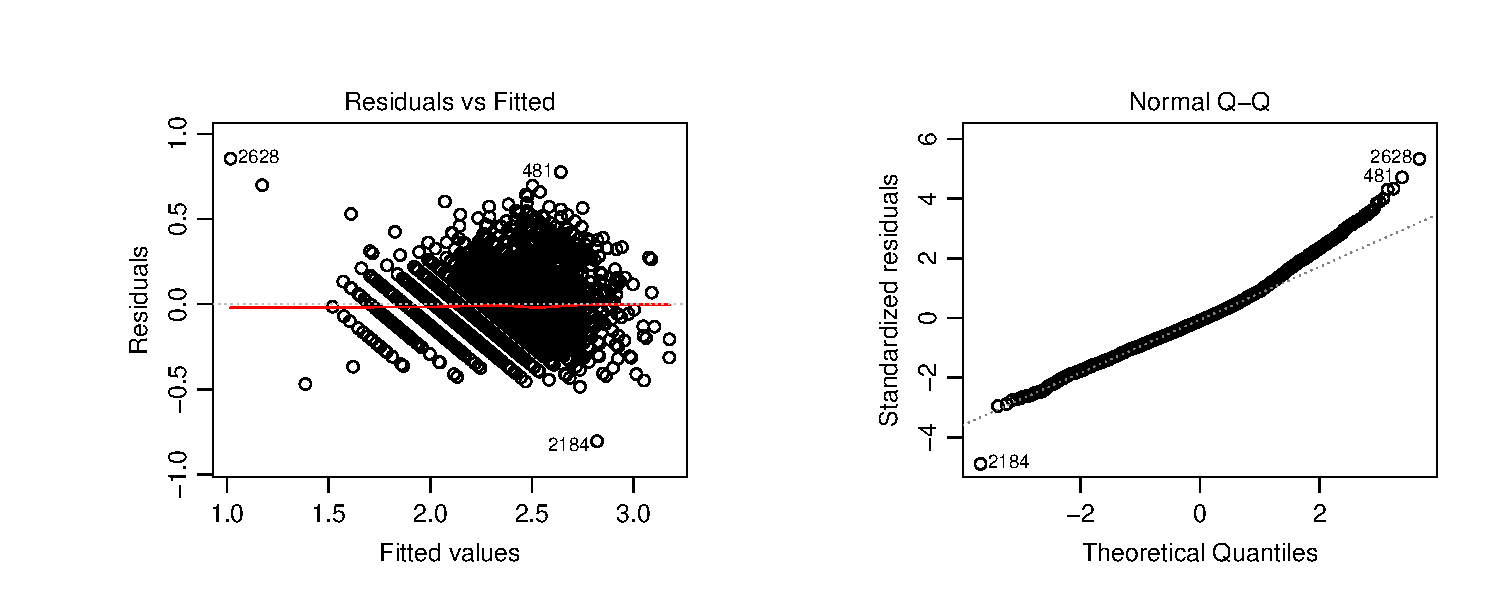
\includegraphics[width = 0.99\textwidth]{finalmodelcheck.pdf}
  \caption{Final model assumptions check.}
  \label{fig:finalmodelcheck}
\end{figure}

\subsection{Artificial Neural Network}

\subsection{Model Comparison}

\clearpage
%%%%%%%%%%%%%%%%%%%% Classification %%%%%%%%%%%%%%%%%%%%
\section{Classification}
\label{sec:classification}

%% \begin{enumerate}
%% \item Explain which classification problem you have chosen to solve.
%% \item Apply at least three of the following methods: Decision Trees
%%   (as in Fig.~\ref{fig:decision_tree}), Logistic/Multinomial
%%   Regression (as in Lst.~\ref{lst:logistic_regression}), K-Nearest
%%   Neighbors (KNN), Naı̈ve Bayes and Artificial Neural Networks (ANN).
%%   (Use cross-validation to select relevant parameters in an inner
%%   cross-validation loop and give in a table the performance results
%%   for the methods evaluated on the same cross-validation splits on the
%%   outer cross-validation loop, i.e. you should use two levels of
%%   cross-validation).
%% \item For the models you are able to interpret explain how a new data
%%   observation is classified.  (If you have multiple models fitted,
%%   (i.e., one for each cross-validation split) either focus on one of
%%   these fitted models or consider fitting one model for the optimal
%%   setting of the parameters estimated by cross-validation to all the
%%   data.)
%% \item Statistically compare the performance of the two best performing
%%   models (i.e., use a paired t-test). Compare in addition if the
%%   performance of your models are better than simply predicting all
%%   outputs to be the largest class in the training data.
%% \end{enumerate}

%% There are two important aspects of classification and regression
%% methods, how well the methods can predict unlabeled data and how well
%% the method describe what aspects in the data causes the data to be
%% classified a certain way.

\subsection{Clasification problem for the dataset}  %%%%%%%%%%%%%%%%%%%%%%%%%%%%%%%%%%%%%%%%
The classification problem for the dataset is to predict the age range
of abalones using their measured physical characteristics.  Age in
years as an attribute can be calculated from the Rings attribute as
Age = 1.5 + Rings.  The original distribution of the Age attribute and
is presented in Fig.~\ref{fig:age_grouping}a.

\begin{figure}[htbp]
  \centering 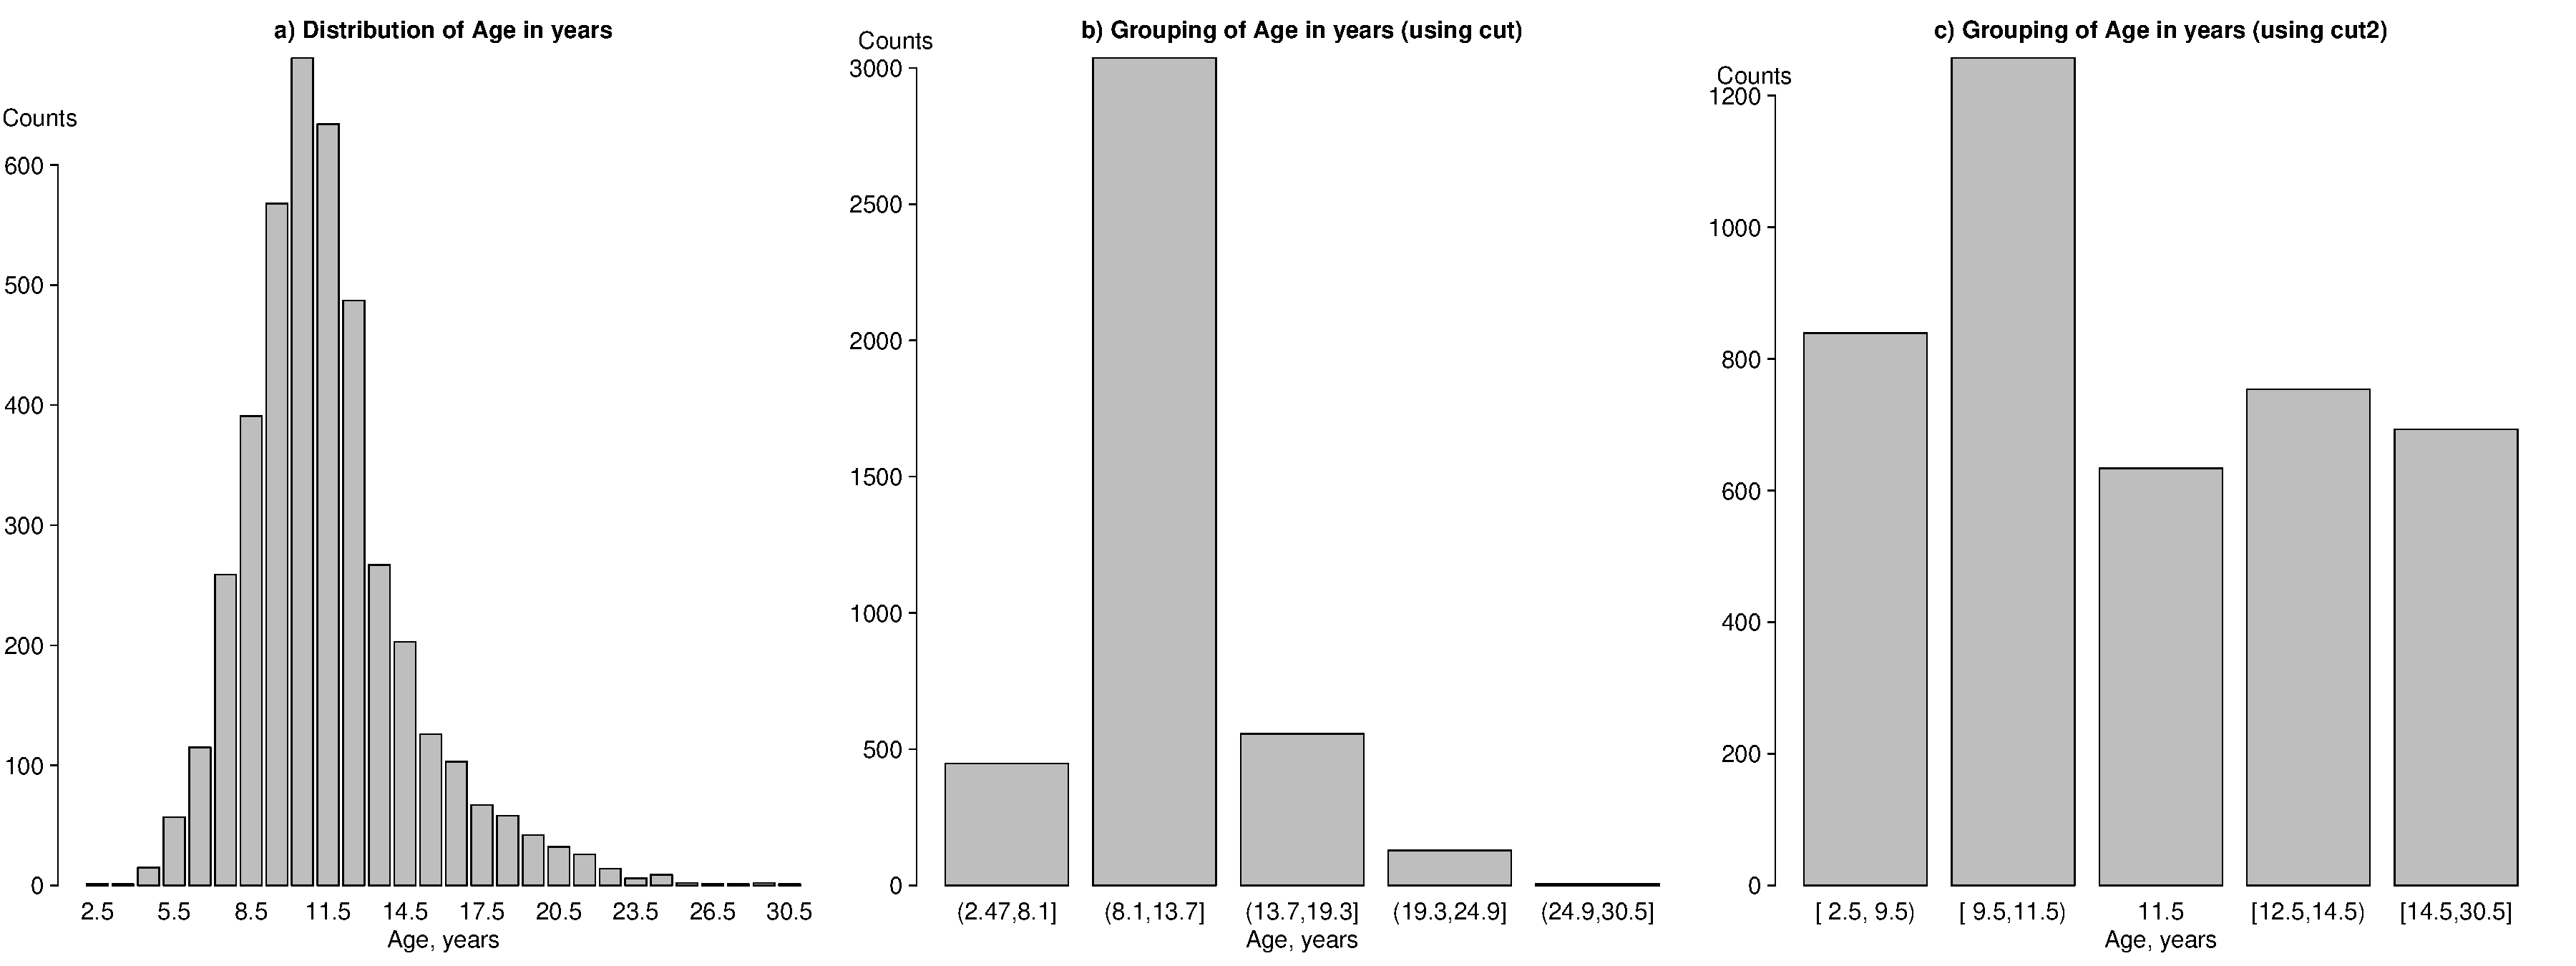
\includegraphics[width =
    0.99\textwidth]{age_grouping.pdf} \cprotect\caption{a) Original
    distribution of the Age attribute derived from Rings attribute as
    Age = 1.5 + Rings.  b) Equal length splitting of the original Age
    attribute using \verb|R cut| function.  c) Quantile groups
    splitting of the original Age attribute using \verb|R cut2|
    function.}
  \label{fig:age_grouping}
\end{figure}

To formulate a classification problem, the continuous Age attribute
has to be splitted into several groups.  There are different ways to
perform this grouping --- either dividing the Age interval into pieces
of equal length as shown in Fig.~\ref{fig:age_grouping}b using the
standard \verb|cut| function in \verb|R|, or dividing the interval
into quantile groups as shown in Fig.~\ref{fig:age_grouping}b using
the function \verb|cut2|.  The advantage of the equal length splitting
is that it mostly retains the original distribution of the Age
attribute, whereas the quantile groups splitting results in a lot more
uniform distribution.  From the perspective of the classification
problem, when a dominant class is present in the dataset with a huge
number of counts compared to other classes, even a ``null'' largest
class classifier will have a decent error rate.  However we are not
supposed to solve class imbalance problems in this particular report,
so we will proceed with predicting the Age range using the equal
length splitting, and then compare the obtained results to the ones
for quantile groups splitting.

\subsection{Applying different methods to solve classification problem}
\subsubsection{Decision trees} %%%%%%%%%%%%%%%%%%%%%%%%%%%%%%%%%%%%%%%%
Decision tree (DT) is a tool that uses a tree-like model of decisions
and their possible consequences.  The goal of applying a decision tree
to the data is to find out how, on the basis of all other attributes,
to classify the age according to splitting in
Fig.~\ref{fig:age_grouping}b.

The complexity of the decision tree model is defined by its complexity
parameter $cp$.  Generally, a full decision tree with $cp = 0$ results
in overfitting --- it has a very low error rate on the training
dataset, but a very large error on the test dataset.  Adjusting the
value of complexity parameter with one layer K-fold cross-validation
is performed in the following way: the data is splitted K times into
non-overlapping test and train datasets, and the number of
observations in the test dataset is N / K, where N is the total number
of observations.  The full decision tree with $cp = 0$ is fitted to
the train data, and then the obtained tree is pruned using a certain
vector of complexity parameters.  At each of the pruning levels, the
pruned tree is used to predict the classes of the test dataset, and
the classification error is calculated.  Averaging over K splits of
data, the plot of the generalization error as a function of the
complexity parameter allows to find the best model suggested by K-fold
cross-validation.  The result of applying one-layer 10-fold
cross-validation for decision tree model selection to the data is
presented in Fig.~\ref{fig:decision_trees}a.  Minimum number of
observations in the node to attempt splitting was set to 5.  The
estimated optimal value of the complexity parameter is 0.00263 and the
error rate is 22.6 \%.  As Fig.~\ref{fig:decision_trees}a shows,
adjusting the complexity parameter brings the training and the test
errors virtually to the same scale, which is clearly not the case when
$cp = 0$.

\begin{figure}[h!]
  \centering
  \begin{minipage}{0.49\textwidth}
    a)\\
    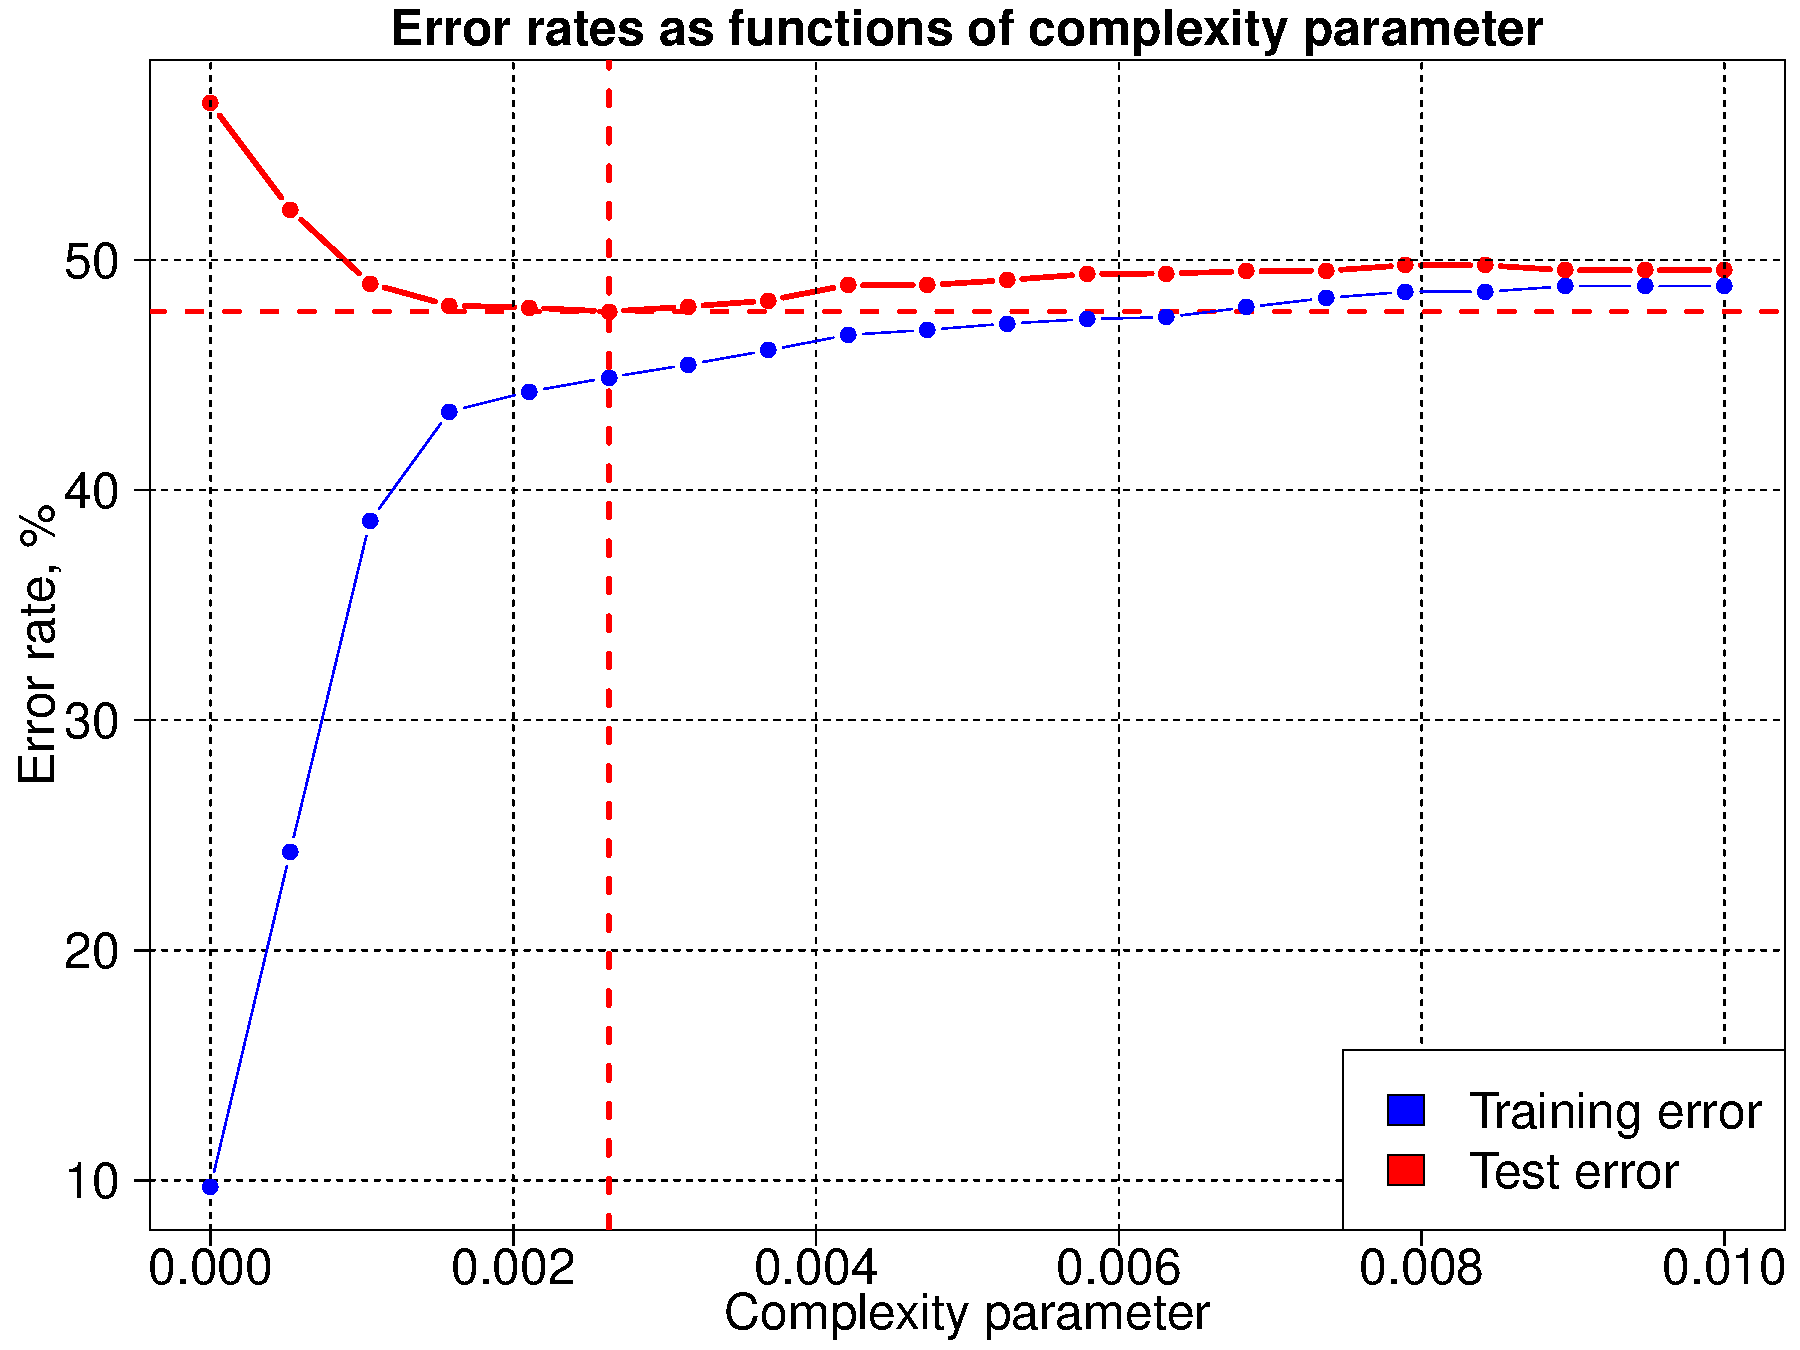
\includegraphics[width = 0.99\textwidth]{decision_tree_err_CV1.pdf}
  \end{minipage} \hfill
  \begin{minipage}{0.49\textwidth}
    b)\\
    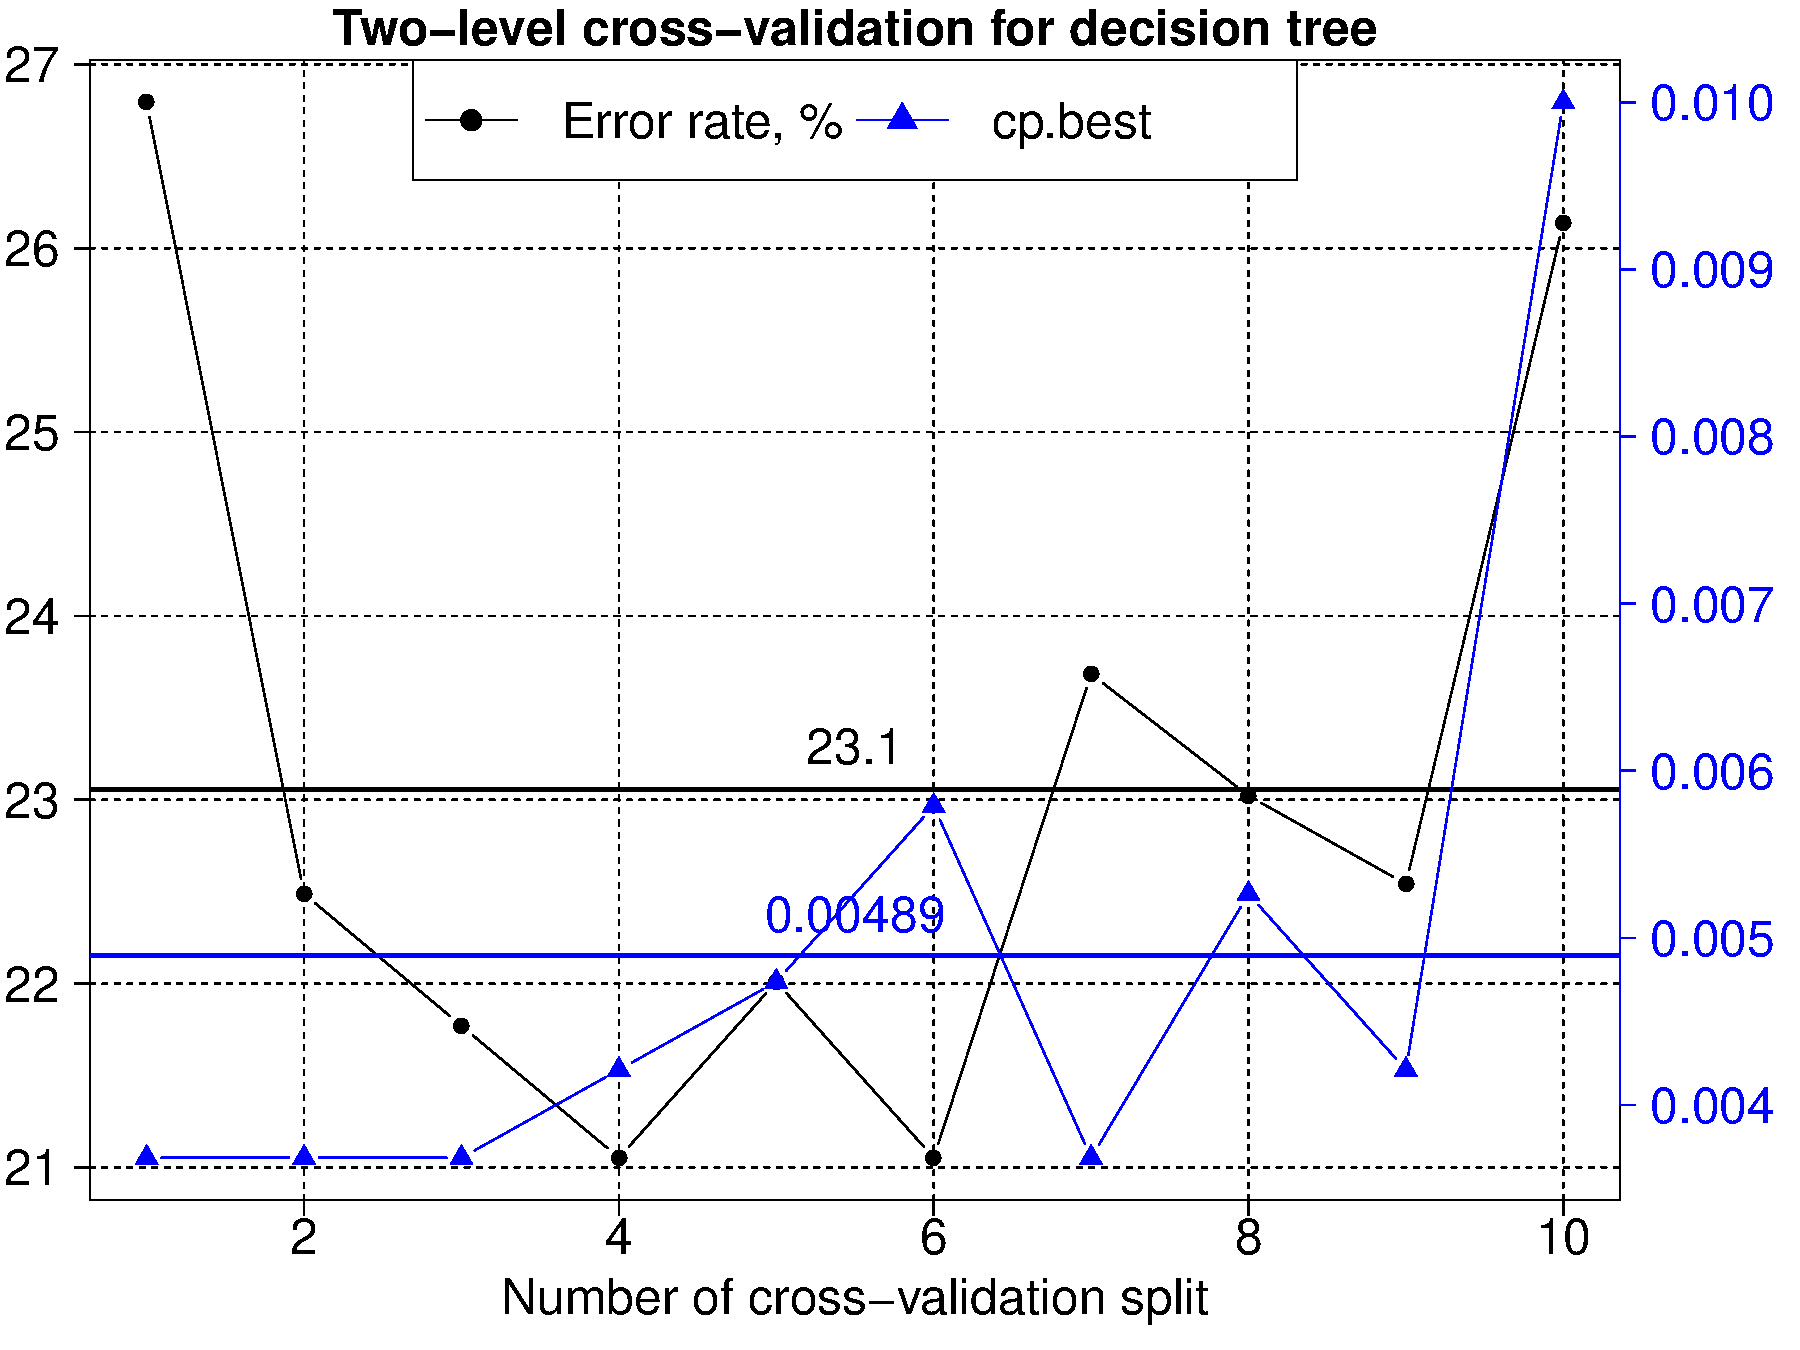
\includegraphics[width = 0.99\textwidth]{decision_tree_CV2.pdf}
  \end{minipage} \vfill
  \begin{minipage}{0.99\textwidth}
    c)\\
    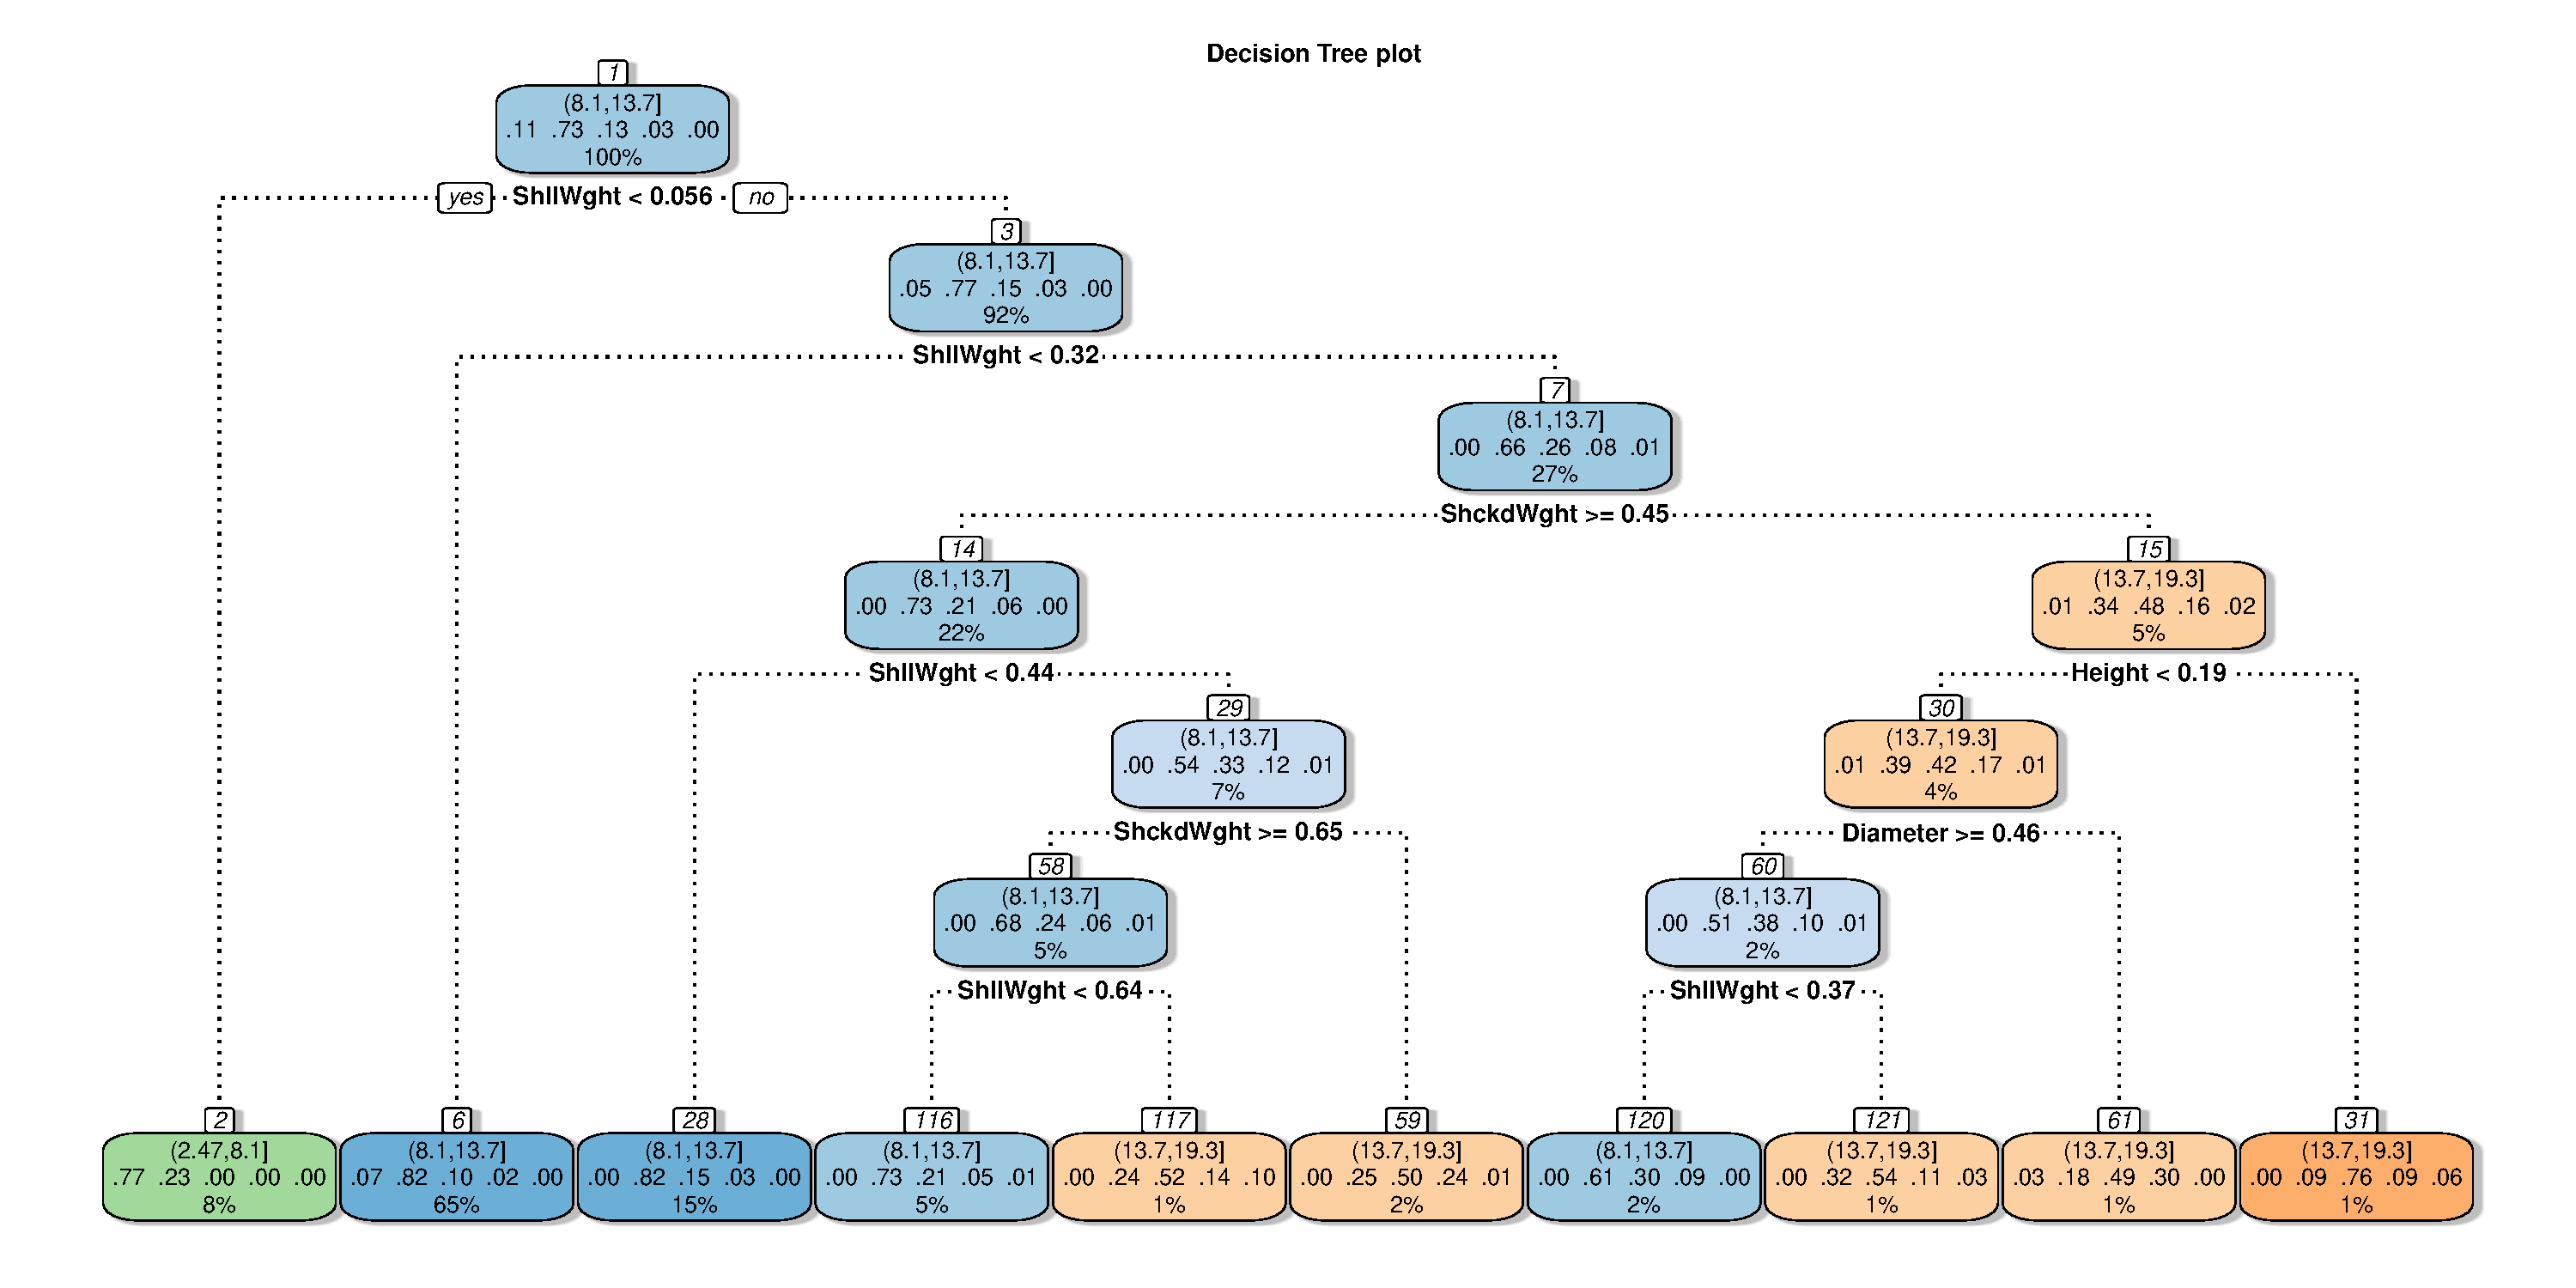
\includegraphics[width = 0.99\textwidth]{decision_tree.pdf}
  \end{minipage} \vfill
  \cprotect\caption{a) One-layer 10-fold cross-validation for decision
    tree model selection.  Minimum number of observations in the node
    to attempt splitting was set to 5.  The optimal pruning level is
    0.00263 and the error rate is 22.6 \%.  b) Two-layer 10 by 10
    cross-validation for decision tree model selection.
    \verb|cp.best| is the complexity parameter value of the best model
    selected in the inner cross-validation loop.  The cross-validated
    generalization error of the decision tree algorithm is $\simeq$
    23.1 \%.  c) Decision tree model with \verb|cp = 0.005| fitted to
    the whole dataset.}
  \label{fig:decision_trees}
\end{figure}

In practice, the one-layer cross-validation for optimal model
selection is combined with the basic cross-validation for estimation
of the generalization error, and that results in the two-layer
cross-validation, that both selects the optimal model and estimates
its generalization error.  The result of applying two-layer 10 by 10
cross-validation for decision tree model selection to the data is
presented in Fig.~\ref{fig:decision_trees}b.  For each of the
cross-validation splits on the outer loop, the error rate of the best
model and the parameter value \verb|cp.best| characterizing the best
model are presented.  So, the error rate or rather the cross-validated
generalization error of the decision tree algorithm is $\simeq$ 23.1
\%.  This result is compared to the performance of other
classification methods in Fig.~\ref{fig:performance}e.

After performing two-layer cross-validation, it is instructive to
interpret the decision tree model by fitting it to the whole dataset.
We chose \verb|cp = 0.005|, and the obtained model is visualized in
Fig.~\ref{fig:decision_trees}c.  The visualization suggests that the
most important decisions are made on the basis of just two attributes
--- \verb|ShllWght| and \verb|ShkcdWght|.  For several relatively
small leaf nodes containing the \verb|(13.7, 19.3]| Age range,
attributes \verb|Height| and \verb|Diameter| are also important.
Taking a new observation, asking the questions suggested by the
decision tree and following the decision instructions defined by the
answers, one can classify it as shown in
Fig.~\ref{fig:decision_trees}c.

\subsubsection{K nearest neighbours}  %%%%%%%%%%%%%%%%%%%%%%%%%%%%%%%%%%%%%%%%
K nearest neighbors (KNN) algorithm is used in pattern recognition for
classification problem.  A nearest neighbor classifier computes the
distance to all data objects, finds the nearest k data objects, and
classifies according to the majority of votes.  The results of
applying two-layer 10 by 10 cross-validation for the k nearest
neighbors model selection is presented in Fig.~\ref{fig:performance}a.
For each of the cross-validation splits on the outer loop, the error
rate of the best model and the parameter value \verb|kNN.best| (the
number of nearest neighbors) characterizing the best model are
presented.  The cross-validated generalization error of the k nearest
neighbors algorithm is $\simeq$ 22.9 \%.  This result is compared to
the performance of other classification methods in
Fig.~\ref{fig:performance}e.

\subsubsection{Naive Bayes}  %%%%%%%%%%%%%%%%%%%%%%%%%%%%%%%%%%%%%%%%
Naive Bayes (NB) classifiers are a family of simple probabilistic
classifiers based on applying Bayes' theorem with strong (naive)
independence assumptions between the features.  The results of
applying two-layer 10 by 10 cross-validation for the naive Bayes
algorithm is presented in Fig.~\ref{fig:performance}b.  On all the
splits, the default model was used with the provided \verb|naiveBayes|
function and standard model parameters \verb|distribution = "normal"|
and \verb|prior = "empirical"|.  The cross-validated generalization
error of the naive Bayes algorithm is $\simeq$ 45.7 \%.  This result
is compared to the performance of other classification methods in
Fig.~\ref{fig:performance}e.

\subsubsection{Artificial Neural Network}  %%%%%%%%%%%%%%%%%%%%%%%%%%%%%%%%%%%%%%%%
Artificial neural networks (ANN) are a family of models inspired by
biological neural networks and are used to estimate or approximate
functions that can depend on a large number of inputs and are
generally unknown.  Artificial neural networks are generally presented
as systems of interconnected ``neurons'' which exchange messages
between each other.  The connections have numeric weights that can be
tuned based on experience, making neural nets adaptive to inputs and
capable of learning.  As with the multinomial regression, the
artificial neural network can be extended for multi-class
classification problem using the softmax function.  The results of
applying two-layer 10 by 10 cross-validation for the artificial neural
network model selection is presented in Fig.~\ref{fig:performance}c.
For each of the cross-validation splits on the outer loop, the error
rate of the best model and the parameter value
\verb|HHiddenUnits.best| (the number of hidden units in the single
hidden layer of the network) characterizing the best model are
presented.  The cross-validated generalization error of the artificial
neural network model is $\simeq$ 21.1 \%.  We limited ourselves to
maximum 5 hidden units in the model. This result is compared to the
performance of other classification methods in
Fig.~\ref{fig:performance}e.  The model containing 4 hidden units, as
suggested by Fig.~\ref{fig:performance}c, fitted to the whole data is
visualized in Fig.~\ref{fig:ANN}.

\begin{figure}[h!]
  \centering
  \begin{minipage}{0.75\textwidth}
    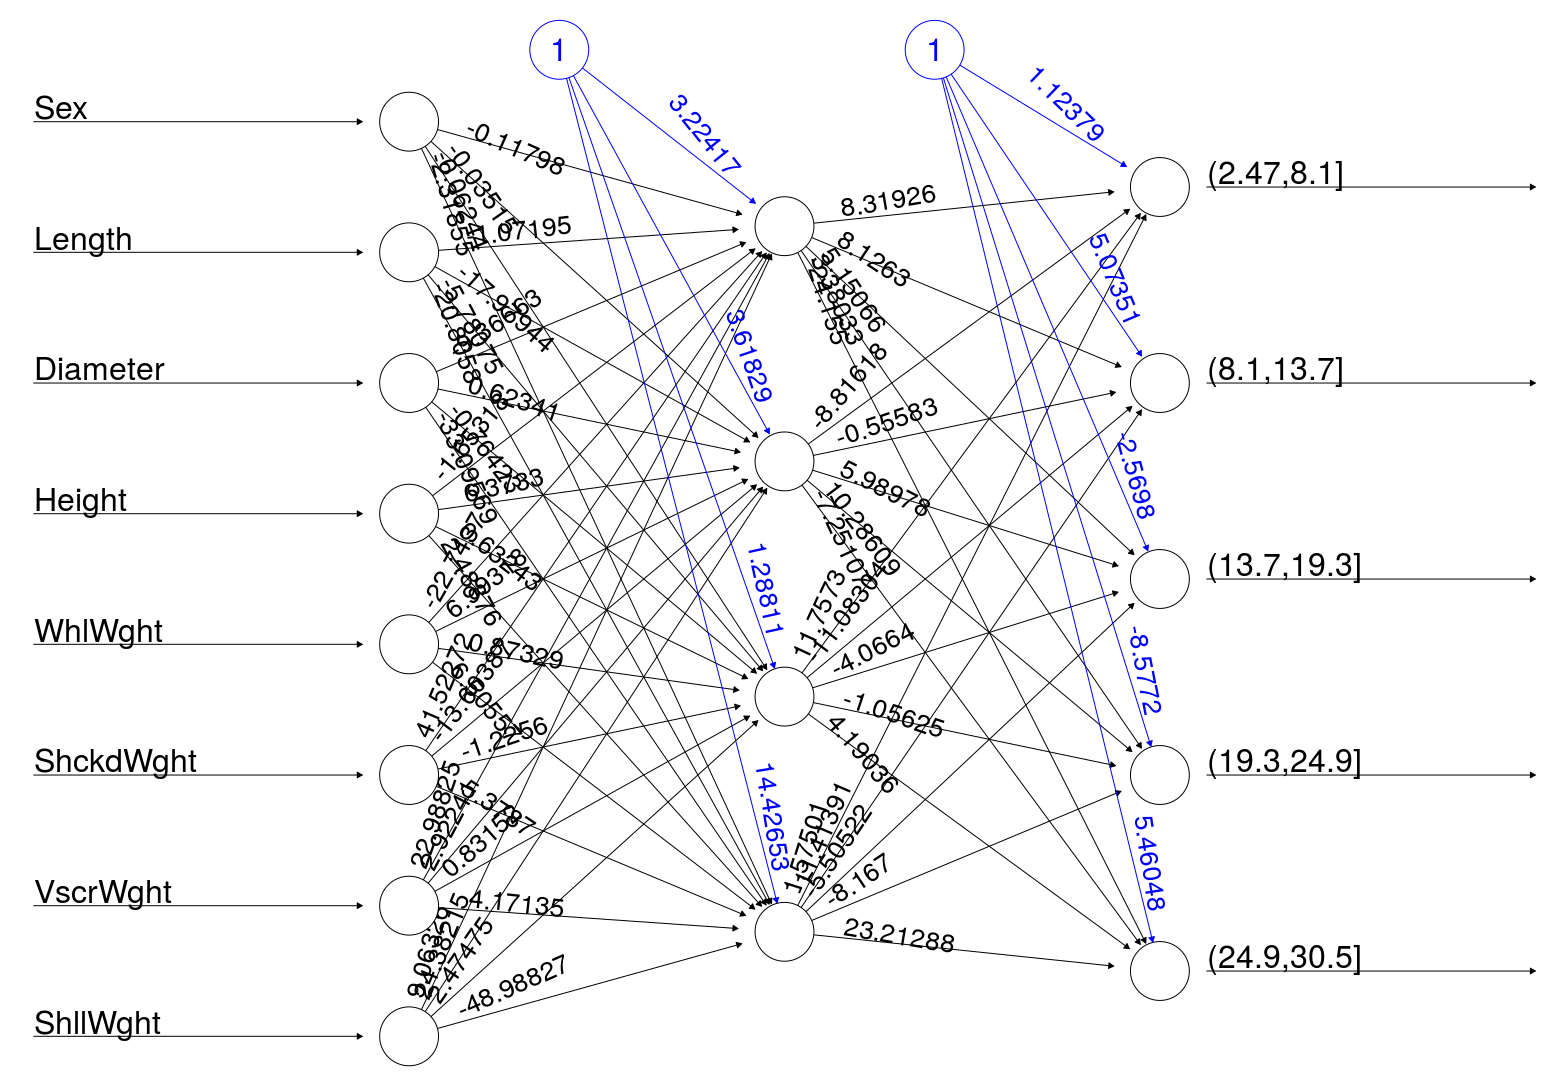
\includegraphics[width = 0.99\textwidth]{ANN.png}
  \end{minipage} \vfill
  \caption{The visualization of the artificial neural network model
    containing 4 hidden units, fitted to the whole data.}
  \label{fig:ANN}
\end{figure}

\subsubsection{Multinomial regression}  %%%%%%%%%%%%%%%%%%%%%%%%%%%%%%%%%%%%%%%%
The basic linear regression model can be extended using the binomial
cost function and the logit link function to the logistic regression
model.  The logistic regression model can be used for classification,
but it is capable do distinguish only between two classes.  The
extension of the logistic regression by using the softmax function
results in the ability to distinguish between more than two classes,
and the model is then called the multinomial regression model (MNMR).
The results of applying two-layer 10 by 10 cross-validation for the
multinomial regression model is presented in
Fig.~\ref{fig:performance}d.  No parameters of the model were tuned in
the inner cross-validation loop (tuning was not discussed in the
lectures or excercises).  The cross-validated generalization error of
the multinomial regression model is $\simeq$ 21.6 \%.  This result is
compared to the performance of other classification methods in
Fig.~\ref{fig:performance}e.

\subsubsection{Performance comparison of the considered methods}
Fig.~\ref{fig:performance}e shows the comparison of cross-validation
generalization errors of the considered classification methods.  ANN
and MNMR show the best results, and NB --- the worst.  If exactly the
same analysis as described above is performed using the alternative
quantile groups splitting as shown in Fig.~\ref{fig:age_grouping}c,
then the performance table for the methods looks like in
Fig.~\ref{fig:performance}d.  Again, ANN and MNMR show the best
results, and NB is the worst, but the error rate of all methods except
NB becomes effectively twice as large.

\begin{figure}[h!]
  \begin{minipage}{0.49\textwidth}
    a)\\
    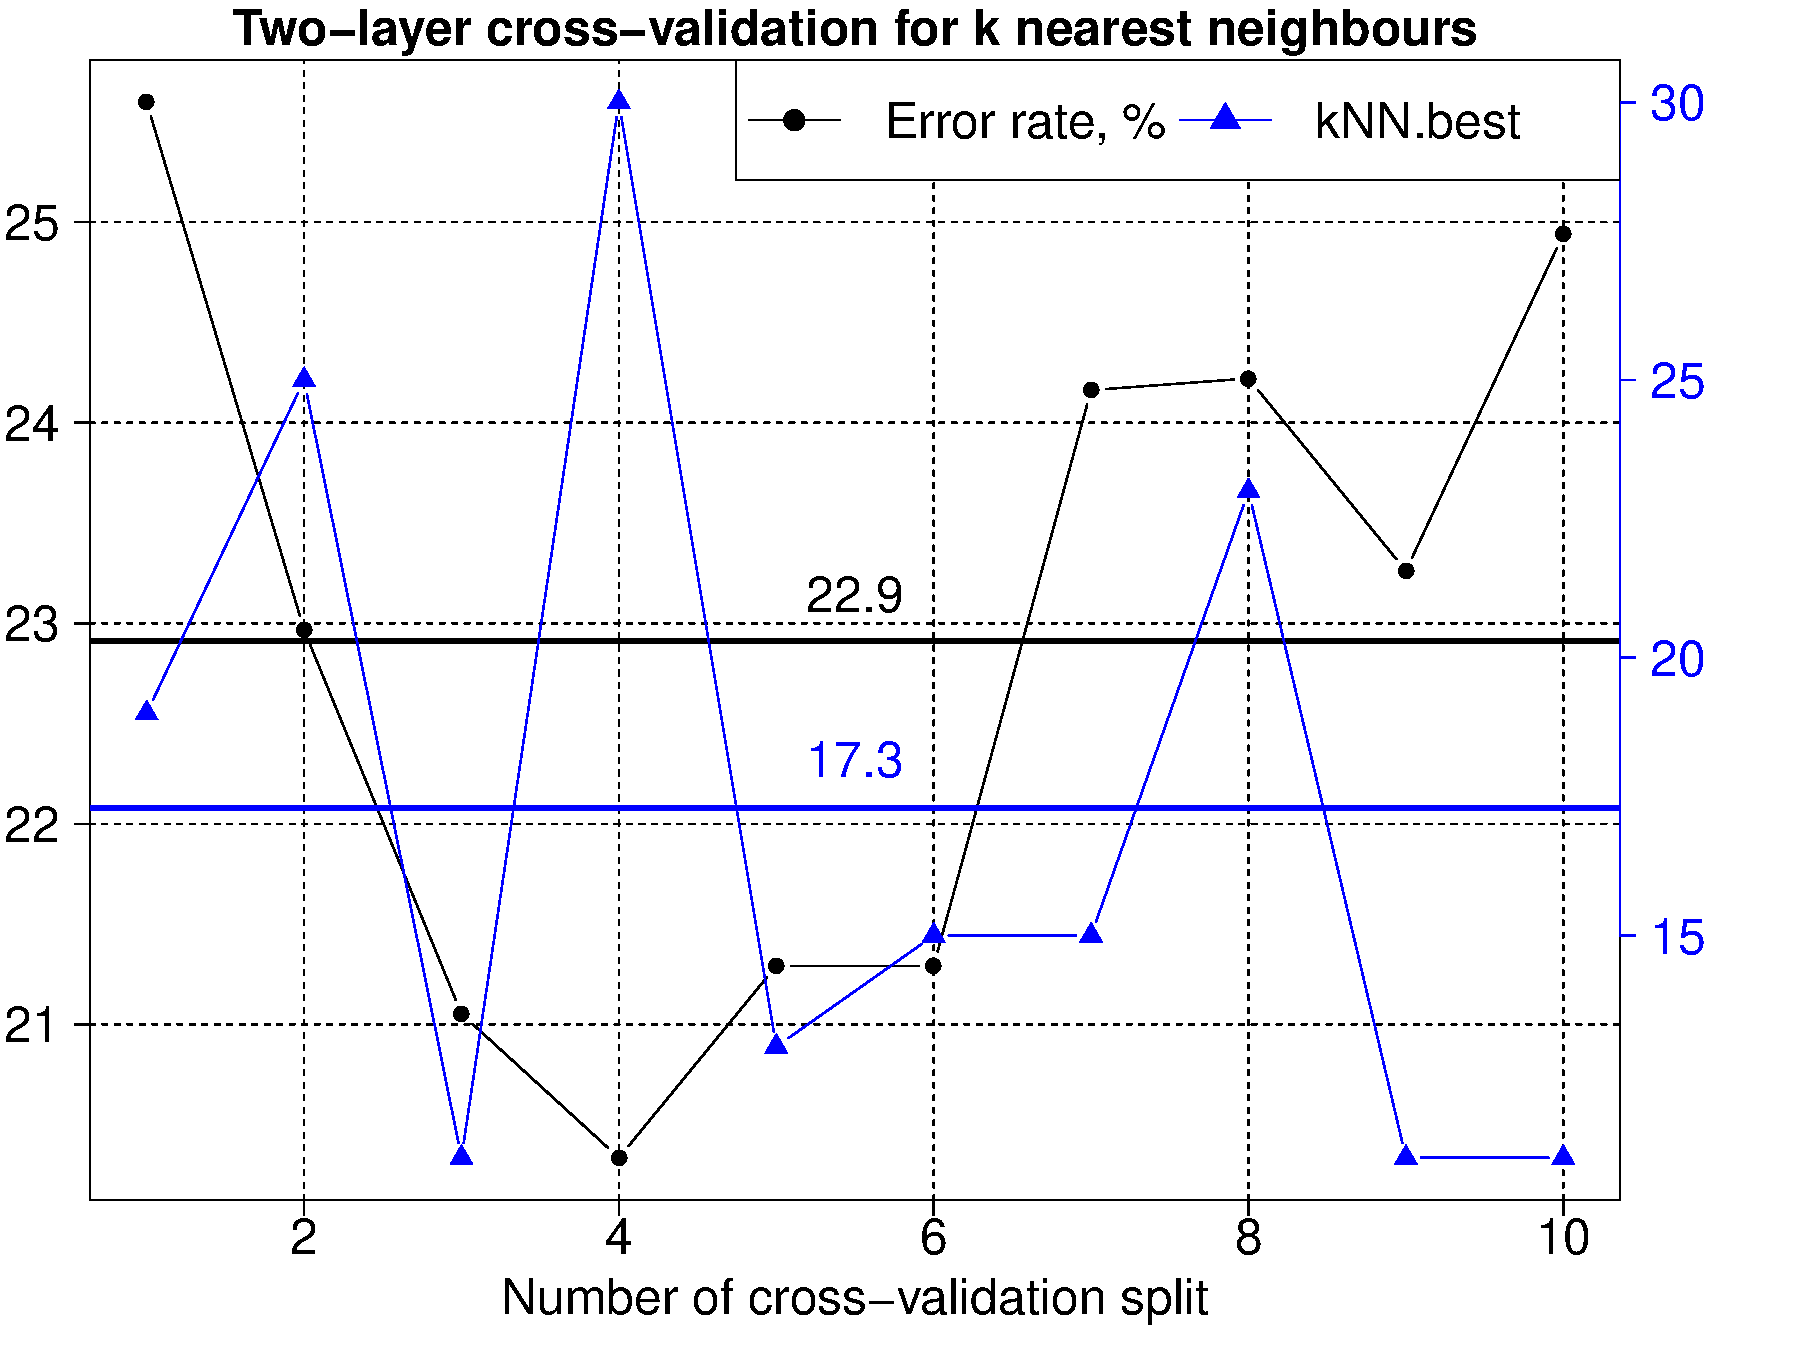
\includegraphics[width = 0.99\textwidth]{k_nearest_neighbors_CV2.pdf}
  \end{minipage} \hfill
  \begin{minipage}{0.49\textwidth}
    b)\\
    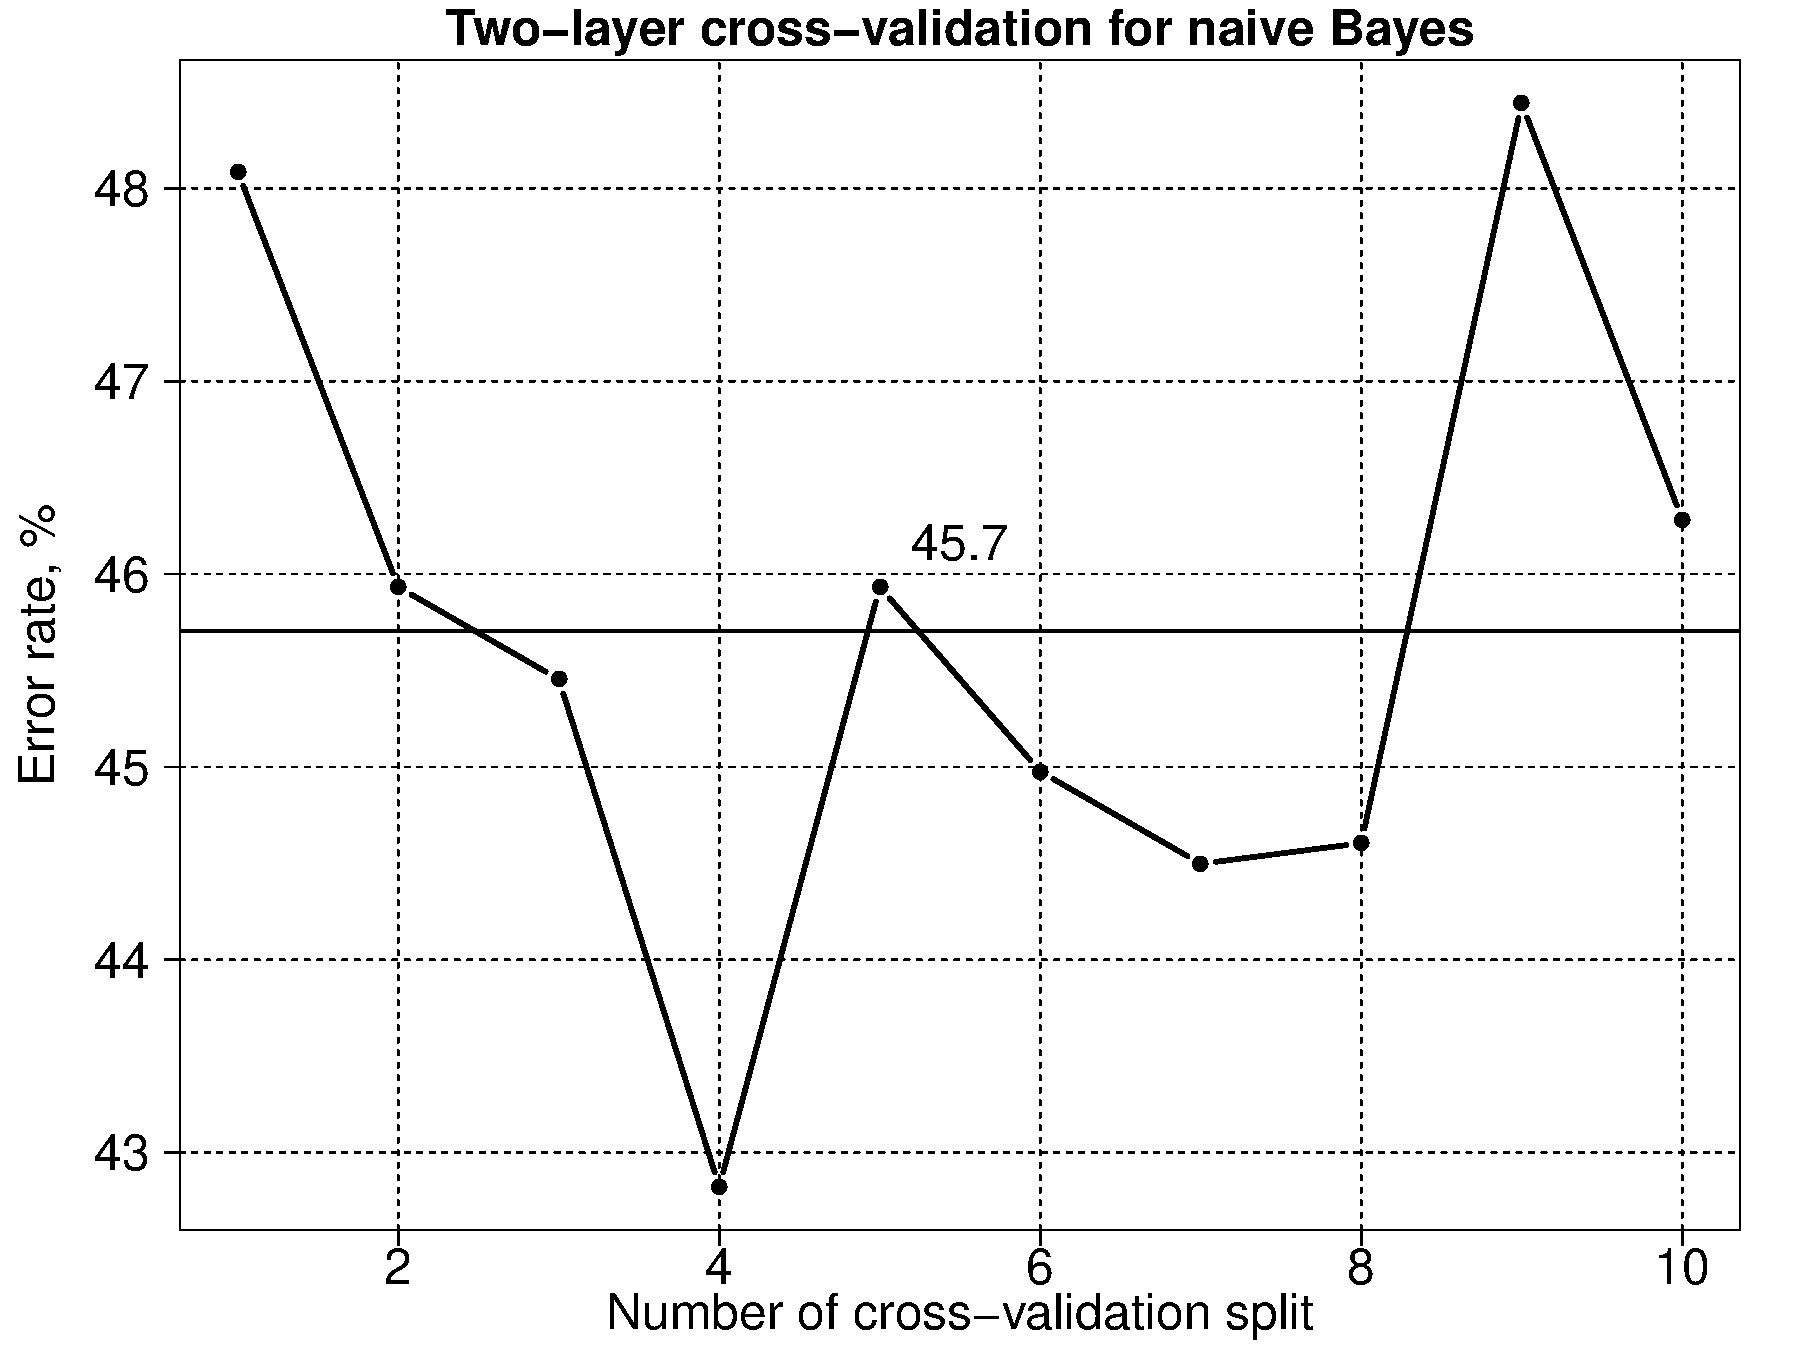
\includegraphics[width = 0.99\textwidth]{naive_bayes_CV1.pdf}
  \end{minipage} \vfill
  \begin{minipage}{0.49\textwidth}
    c)\\
    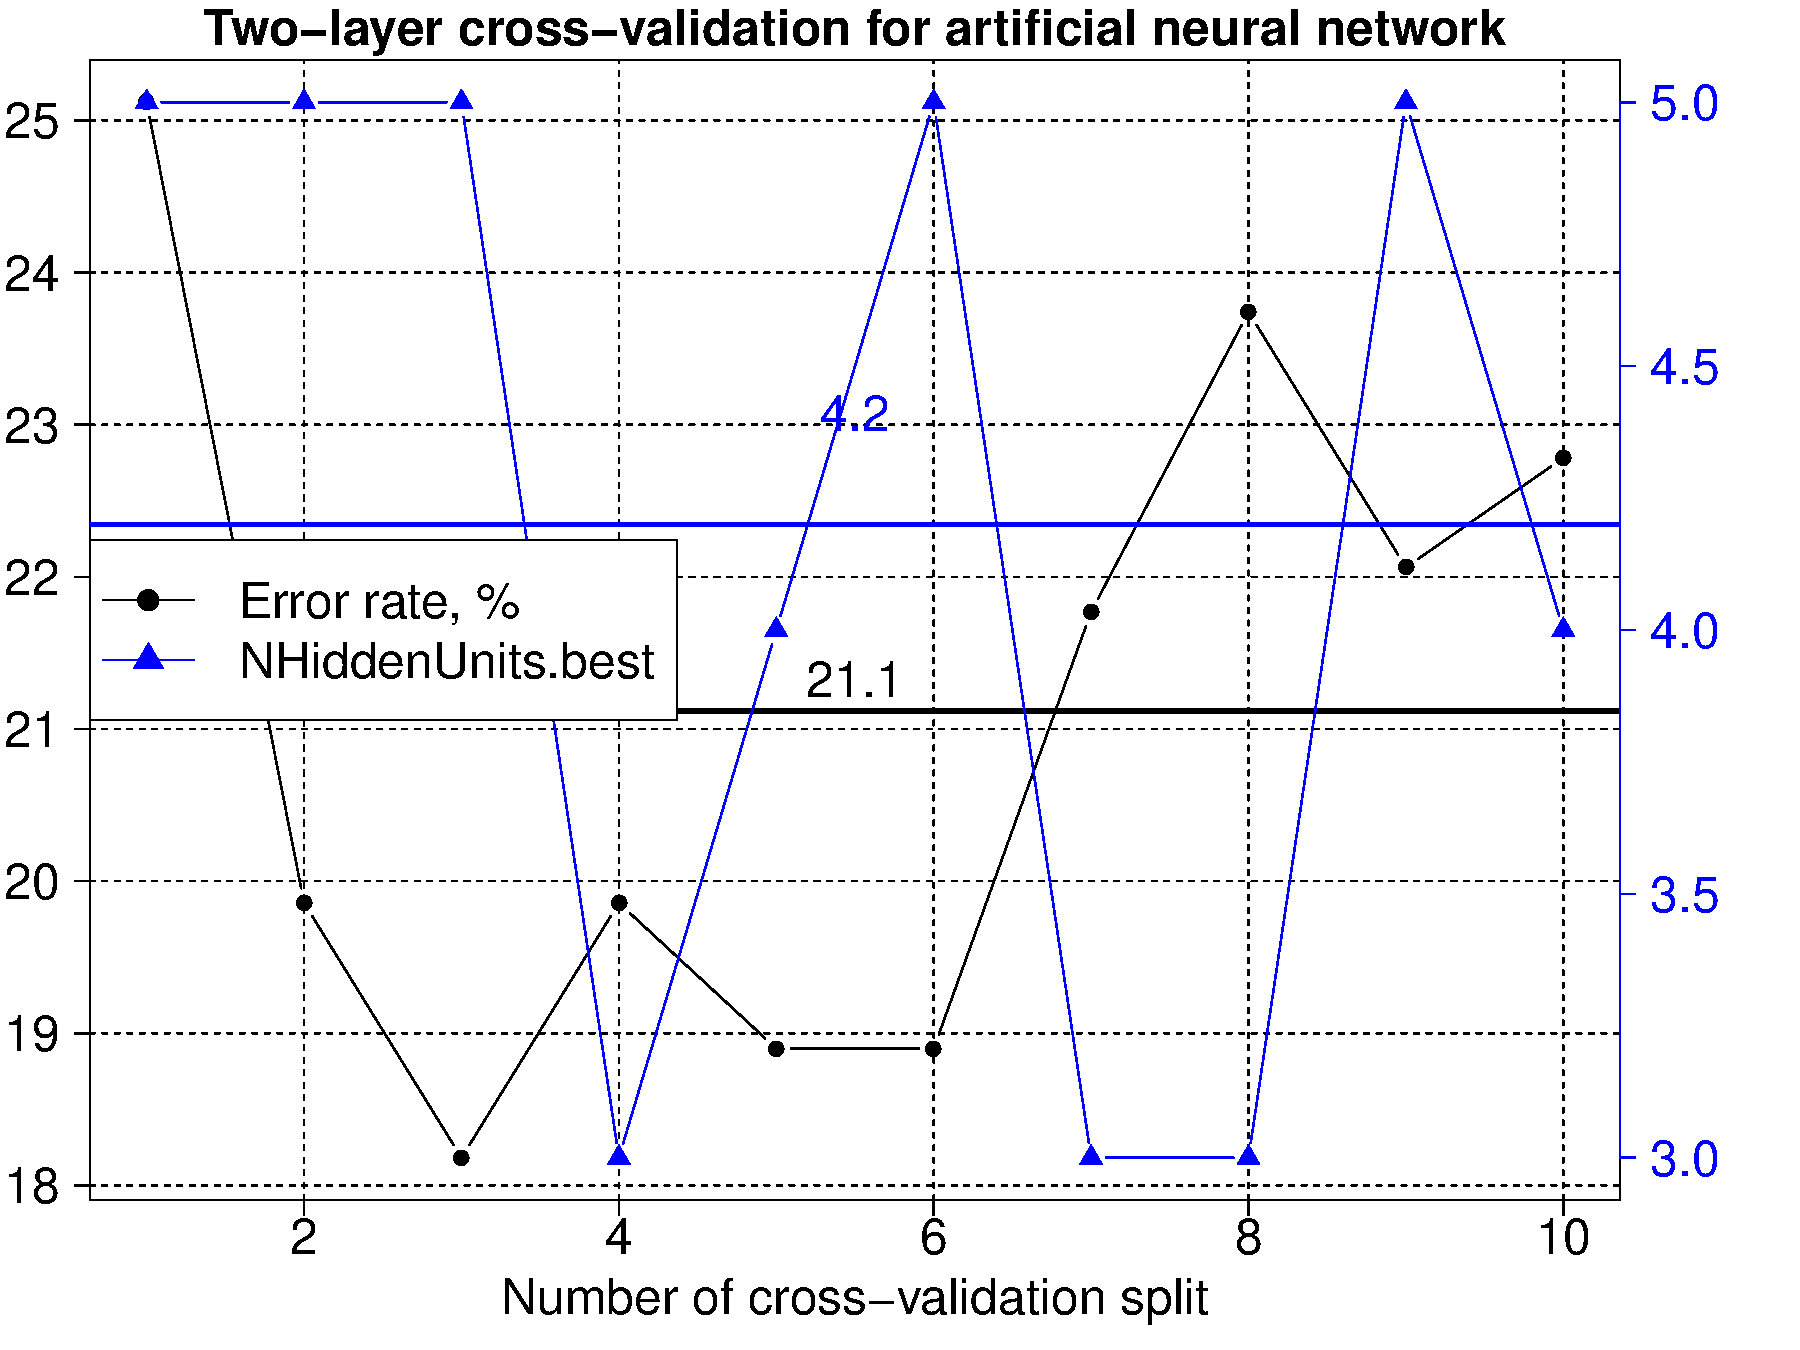
\includegraphics[width = 0.99\textwidth]{artificial_neural_network_CV2.pdf}
  \end{minipage} \hfill
  \begin{minipage}{0.49\textwidth}
    d)\\
    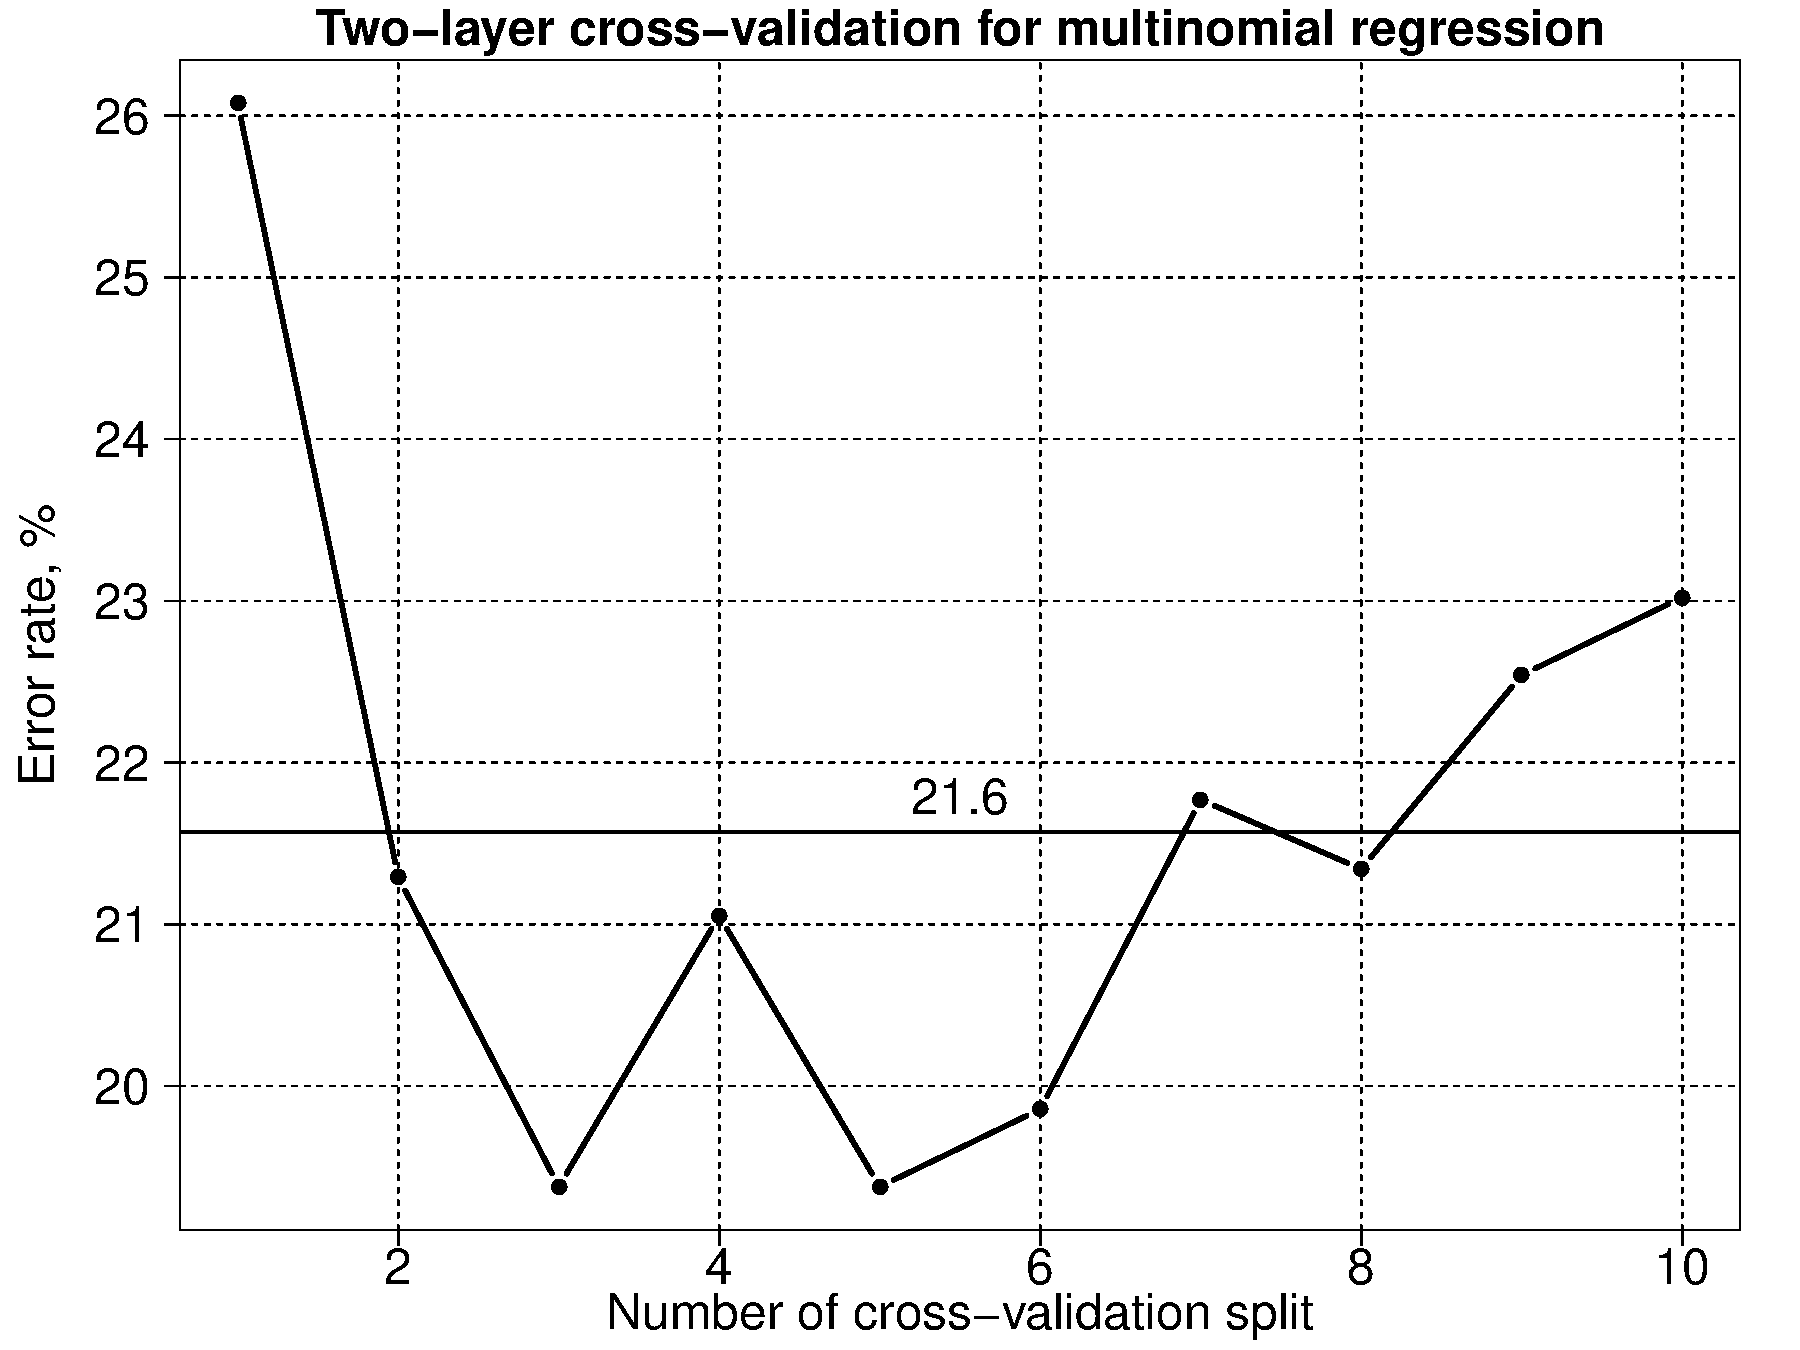
\includegraphics[width = 0.99\textwidth]{multinomial_regression_CV1.pdf}
  \end{minipage} \vfill
  \begin{minipage}{0.49\textwidth}
    e) Equal length splitting using \verb|cut|\\
    \begin{center}
    \begin{tabular}{c|c|c|c|c|c}
      \toprule
      Method & DT & KNN & NB & ANN & MNMR\\
      \midrule
      Error rate, \% & 23.1 & 22.9 & {\color{red} 45.7} & {\color{green} 21.1} & {\color{green} 21.6}\\
      \bottomrule
    \end{tabular}
    \end{center}
  \end{minipage} \hfill
  \begin{minipage}{0.49\textwidth}
    f) Group quantiles splitting using \verb|cut2|\\
    \begin{center}
      \begin{tabular}{c|c|c|c|c|c}
        \toprule
        Method & DT & KNN & NB & ANN & MNMR\\
        \midrule
        Error rate, \% & 47.5 & 49.2 & {\color{red} 54.4} & {\color{green} 45.8} & {\color{green} 46.4}\\
        \bottomrule
      \end{tabular}
    \end{center}
  \end{minipage} \hfill
  \cprotect\caption{a) Two-layer 10 by 10 cross-validation for the k
    nearest neighbors (KNN) model selection.  \verb|kNN.best| is the
    number of neighbors parameter value of the best model selected in
    the inner cross-validation loop.  b) Two-layer 10 by 10
    cross-validation for the naive Bayes (NB) algorithm.  On all the
    splits, the default model was used with the provided
    \verb|naiveBayes| function and standard model parameters
    \verb|distribution = "normal"| and \verb|prior = "empirical"|.  c)
    Two-layer 10 by 10 cross-validation for the artificial neural
    network (ANN) model selection.  \verb|NHiddenUnits.best| is the
    number of hidden units parameter value of the best model selected
    in the inner cross-validation loop.  d) Two-layer 10 by 10
    cross-validation for the multinomial regression model (MNMR). No
    parameters of the model were tuned in the inner cross-validation
    loop (tuning was not discussed in the lectures or excercises). e)
    Comparison of cross-validated generalization errors of the
    considered classification methods for equal length splitting as in
    Fig.~\ref{fig:age_grouping}b.  ANN and MNMR show the best results,
    NB is the worst.  f) Same as e) but for quantile groups splitting
    as in Fig.~\ref{fig:age_grouping}c.  Again, ANN and MNMR show the
    best results, and NB is the worst.}
  \label{fig:performance}
\end{figure}

\subsection{Statistical comparison of two best performing models}
As indicated by both Fig.~\ref{fig:performance}e-f, the two best
performing models are ANN and MNMR models.  We can statistically
compare their performance between each other, as well as with the
``null'' largest class classifier (LCl).  Statistical comparison of
two models is performed in the following way.  The populations of the
error rates of the classifiers are compared using a paired t-test, and
if the difference in their means is significantly non-zero, then one
classifier is better than the other.  The outer layer of the
cross-validation is used to get a sample of generalization errors of
the two models.  Next, if the means of the populations of the error
rates are significantly different, the test-statistic will produce a
very low p-value (p-value $\leq$ 0.05) of the paired t-test, which
under the null hypothesis indicates the probability that the
classifiers are not significantly different.  The populations of the
error rates of Lcl, ANN, and MNMR models are presented in
Fig.~\ref{fig:comparison}.  In parenthesis after ANN and MNMR, the
p-value of the paired t-test comparing the classifier with Lcl is
presented.  The p-value of the t-test comparing ANN with MNMR is
presented separately.

\begin{figure}[h!]
  \begin{minipage}{0.49\textwidth}
    a) Equal length splitting using \verb|cut|\\
    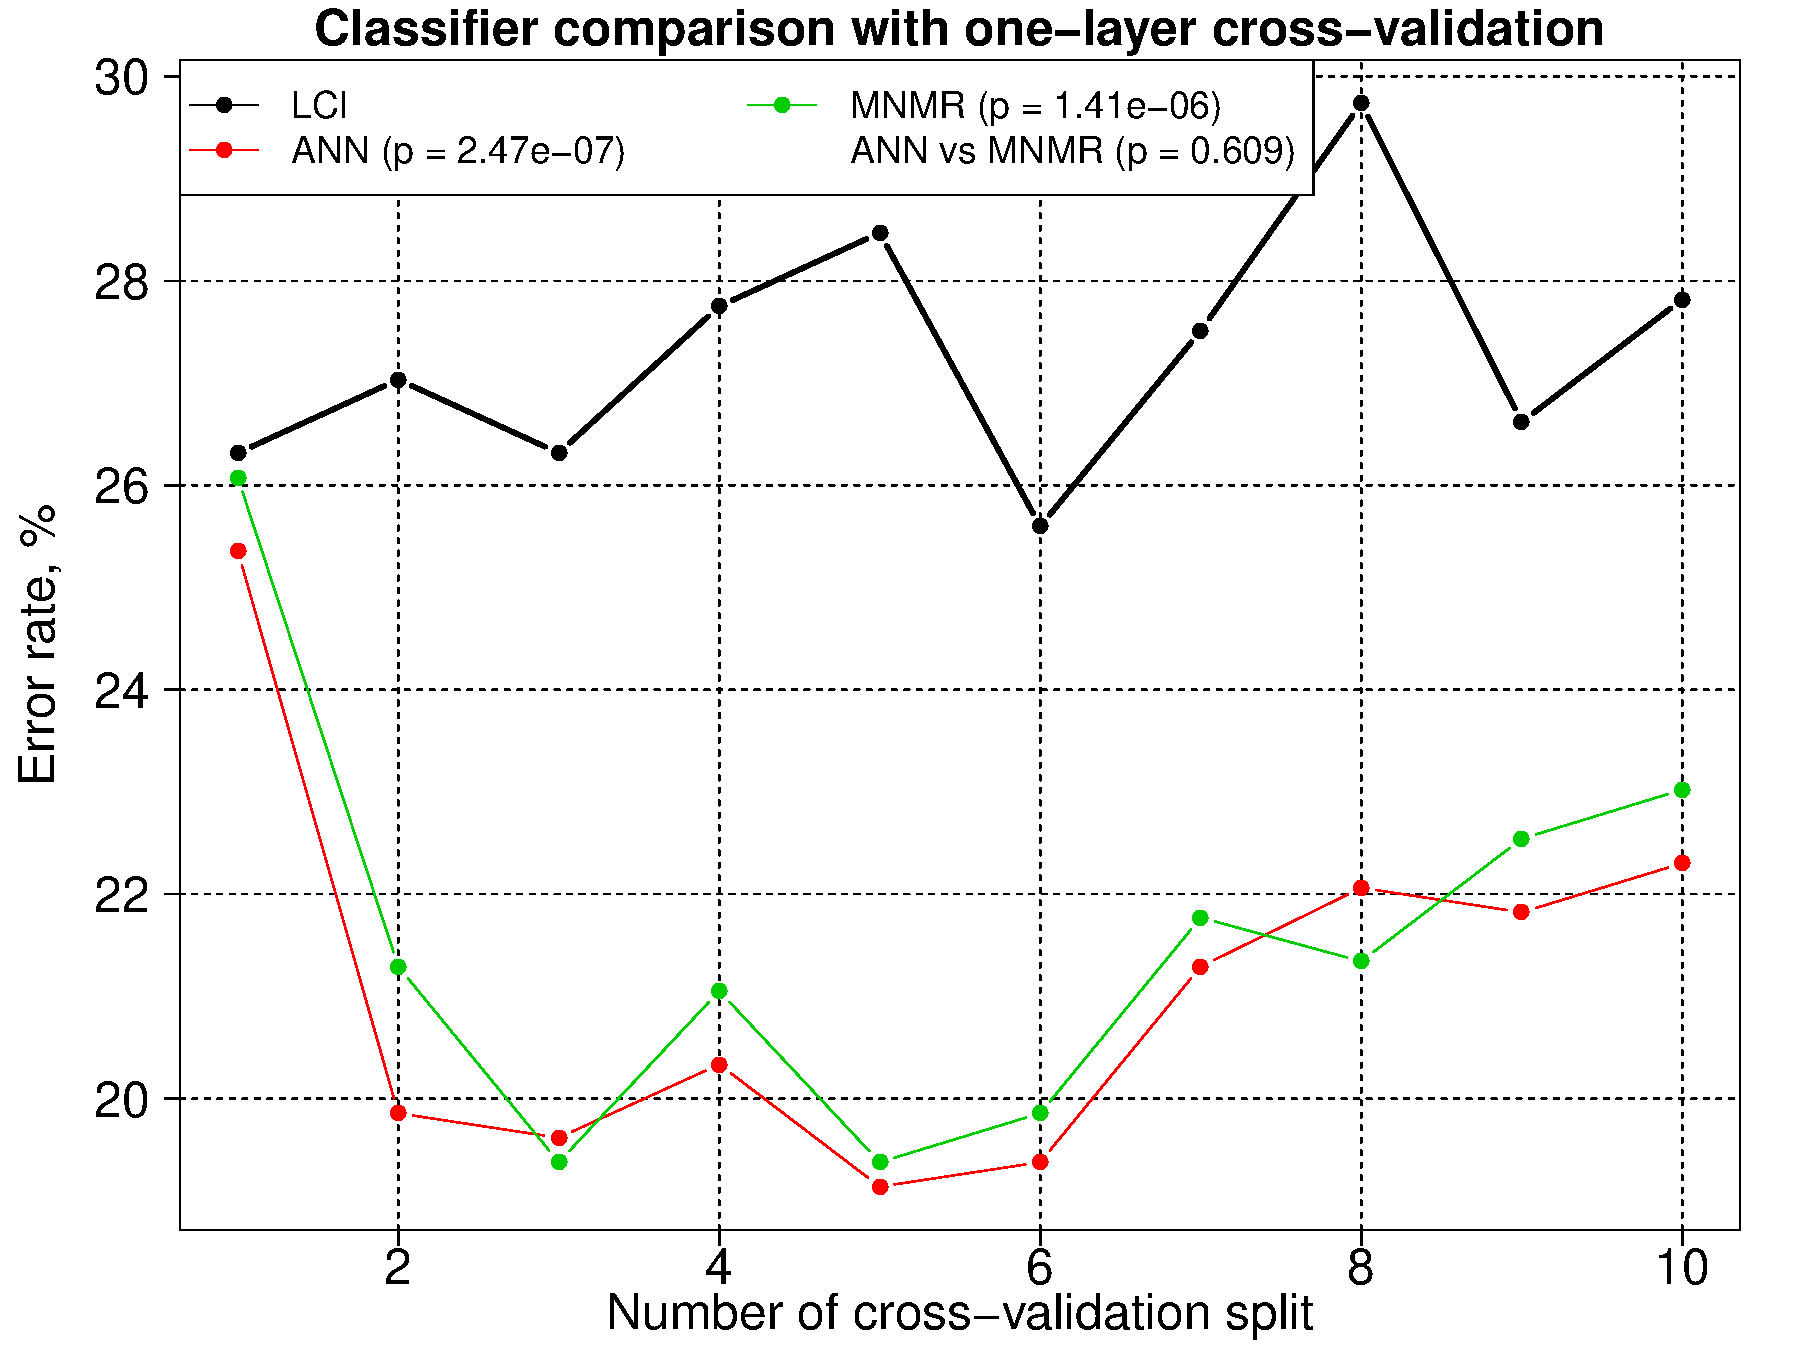
\includegraphics[width = 0.99\textwidth]{classifier_comparison_cut_1.pdf}
  \end{minipage} \hfill
  \begin{minipage}{0.49\textwidth}
    b) Group quantiles splitting using \verb|cut2|\\
    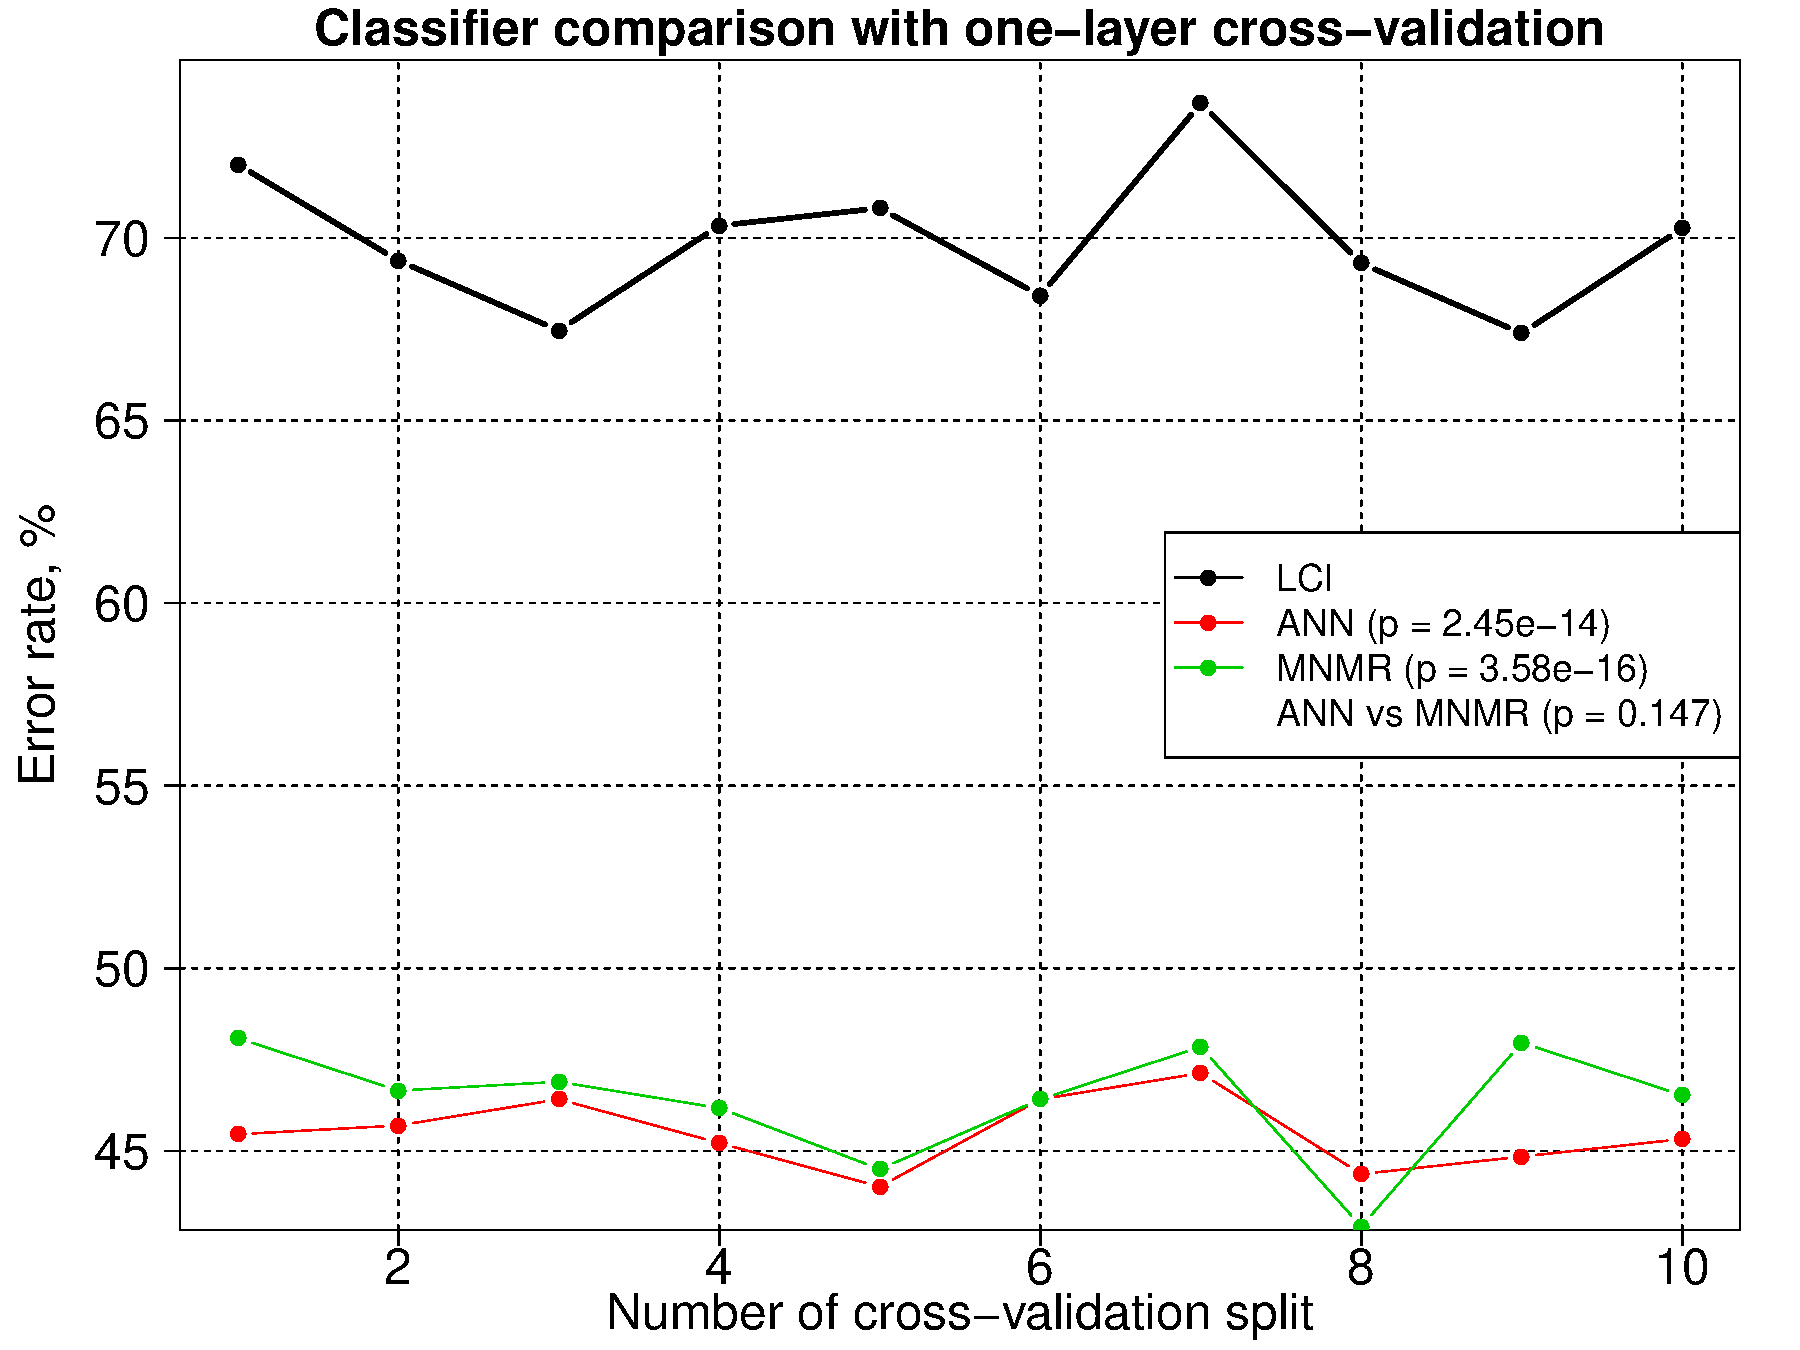
\includegraphics[width = 0.99\textwidth]{classifier_comparison_cut_2.pdf}
  \end{minipage} \vfill
  \caption{The populations of the error rates of Lcl, ANN, and MNMR
    models are presented in Fig.~\ref{fig:comparison}.  In parenthesis
    after ANN and MNMR, the p-value of the paired t-test comparing the
    classifier with Lcl is presented.  The p-value of the t-test
    comparing ANN with MNMR is presented separately. a) Equal length
    splitting of the Age attribute.  b) Group quantiles splitting of
    the Age attribute.}
  \label{fig:comparison}
\end{figure}

Despite the $\simeq$ 2-fold difference in absolute values, for both
Fig.~\ref{fig:comparison}a-b, ANN and MNMR classifiers are
significantly different from the LCl, because corresponding the
p-values of the paired t-tests are extremely low.  At the same time,
we must conclude that for both cases ANN and MNMR are not
significantly different from each other, though the difference is more
obvious in Fig.~\ref{fig:comparison}b than in
Fig.~\ref{fig:comparison}a.

%%%%%%%%%%%%%%%%%%%% Results and Discussion %%%%%%%%%%%%%%%%%%%%
\section{Results and Discussion}
\label{sec:results_and_discussion}

The considered classification problem for the dataset was to predict
the age range of abalones using their measured physical
characteristics.  We have investigated two possible strategies of
splitting the continuous attribute Age into groups --- using equal
length splitting, or quantile groups splitting.  In both cases, the
lowest cross-validated generalization errors were obtained for
artificial neural network (ANN) model and multinomial regression
(MNMR) model, though the classification error rates for the equal
length splitting were 2-fold lower than the error rates for group
quantile splitting.  Statistical comparison of ANN and MNMR using the
paired t-test showed that the classifiers are not significantly
different from each other, but significantly different from the
``null'' largect class classifier.


%% If your data has previously been analyzed by regression or
%% classification in the lit- erature, please report what methods have
%% been used previously as well as their performance and relate your
%% results to these previous results.

%% Notice, if the analysis of your data is too computationally demanding
%% for choosing parameters in the inner cross-validation loop we suggest
%% you use the hold-out method instead of K-fold
%% cross-validation. Furthermore, if analyzing the data by ANN is too
%% computationally demanding you can consider only analyzing a subset of
%% your data by ANN.

%% The report should be 5-10 pages long including figures and tables and
%% give a precise and coherent account of the results of the regression
%% and classification methods applied to your data. Please hand in the
%% report by uploading it as a single, uncompressed .pdf file to
%% CampusNet no later than {\bf 12 April at 13:00}.  To ensure all group
%% members get credit for the report, put your names and study numbers on
%% the front page and ensure you upload the report as a group hand in and
%% put the name of your dataset on the front page.
%%%%%%%%%%%%%%%%%%%% Bibliography %%%%%%%%%%%%%%%%%%%%
\begin{thebibliography}{99}
\bibitem{Waugh.thesis} S.~Waugh,''Extending and Benchmark
  Cascade-Correlation,'' Thesis, 1997.
\bibitem{Mayukh} H.~Mayukh, ``Age of Abalones using Physical
  Characteristics: A Classification Problem,'' ECE 539 Fall 2010
  Project Report, Department of Electrical and Computer Engineering
  University of Wisconsin-Madison, 2010.
\bibitem{datadescription} \url{http://archive.ics.uci.edu/ml/datasets/Abalone}
\end{thebibliography}
\end{document}

%% \begin{lstlisting}[label = lst:logistic_regression, caption = {Results of logistic regression}]
%%   Call:
%% glm(formula = Class ~ Malaise + Ascites + Bilirubin + Histology, 
%%     family = binomial(link = logit), data = data)

%% Deviance Residuals: 
%%     Min       1Q   Median       3Q      Max  
%% -2.7029   0.2382   0.2888   0.4330   1.8019  

%% Coefficients:
%%             Estimate Std. Error z value Pr(>|z|)   
%% (Intercept)   1.2874     0.8407   1.531  0.12567   
%% Malaise       0.9020     0.5670   1.591  0.11162   
%% Ascites       1.9074     0.6621   2.881  0.00397 **
%% Bilirubin    -0.7838     0.2613  -3.000  0.00270 **
%% Histology    -0.9933     0.6132  -1.620  0.10529   
%% ---
%% Signif. codes:  0 ‘***’ 0.001 ‘**’ 0.01 ‘*’ 0.05 ‘.’ 0.1 ‘ ’ 1

%% (Dispersion parameter for binomial family taken to be 1)

%%     Null deviance: 145.117  on 144  degrees of freedom
%% Residual deviance:  91.903  on 140  degrees of freedom
%%   (10 observations deleted due to missingness)
%% AIC: 101.9

%% Number of Fisher Scoring iterations: 5
%% \end{lstlisting}
